\documentclass[journal,twoside,web]{ieeecolor}
\usepackage{xcolor}
\usepackage{jsen}
\usepackage{cite}
\usepackage{amsmath,amssymb,amsfonts}
\usepackage{algorithmic}
\usepackage{graphicx}
\usepackage{textcomp}
\usepackage{wrapfig}
\usepackage{xcolor}
\usepackage[normalem]{ulem}
% \usepackage{cite}
\usepackage{array}
\newcolumntype{C}[1]{>{\centering\let\newline\\\arraybackslash\hspace{0pt}}m{#1}}
\usepackage{multirow}
\usepackage[
    backend=biber,
    style=ieee,
    sorting=none,
    url=false,
    doi=false,
    isbn=false
]{biblatex}
\addbibresource{references.bib}
\AtEveryBibitem{%
  \clearfield{note}%
  \clearfield{howpublished}%
}
% omit the fixed 'in' macro used in bibliography
\renewbibmacro{in:}{}

% \def\BibTeX{{\rm B\kern-.05em{\sc i\kern-.025em b}\kern-.08em
%     T\kern-.1667em\lower.7ex\hbox{E}\kern-.125emX}}
% \markboth{\journalname, VOL. XX, NO. XX, XXXX 2024}
% {Author \MakeLowercase{\textit{et al.}}: Preparation of Papers for IEEE TRANSACTIONS and JOURNALS (May 2024)}
\definecolor{abstractbg}{rgb}{0.89804,0.94510,0.83137}
\setlength{\fboxrule}{0pt}
\setlength{\fboxsep}{0pt} 
\newcommand\hl{\bgroup\markoverwith
  {\textcolor{yellow}{\rule[-.5ex]{.1pt}{2.5ex}}}\ULon}
  
\begin{document}
\title{A Near-Field Radio-Frequency System for Continuous Left and Right Lung Volume Sensing}
\author{Aakash~Kapoor,~\IEEEmembership{Student~Member,~IEEE,} Thomas~B.~Conroy,~\IEEEmembership{Student~Member,~IEEE,} Kapil~Gangwar,~\IEEEmembership{Student~Member,~IEEE,} Edwin~C.~Kan,~\IEEEmembership{Senior~Member,~IEEE,} and Joaquin~Araos
\thanks{Research reported in this article was supported by the National Institutes of Health under award 1R21EB034562-01.}
\thanks{AK, TBC, KG, and ECK are with the Department of Electrical and Computer Engineering, Cornell University, Ithaca, NY 14853, USA. JA is with the College of Veterinary Medicine, Cornell University, Ithaca, NY 14853 USA (email: ak2247@cornell.edu)}}

\IEEEtitleabstractindextext{%
\fcolorbox{abstractbg}{abstractbg}{%
\begin{minipage}{\textwidth}%
\begin{wrapfigure}[12]{r}{3in}%
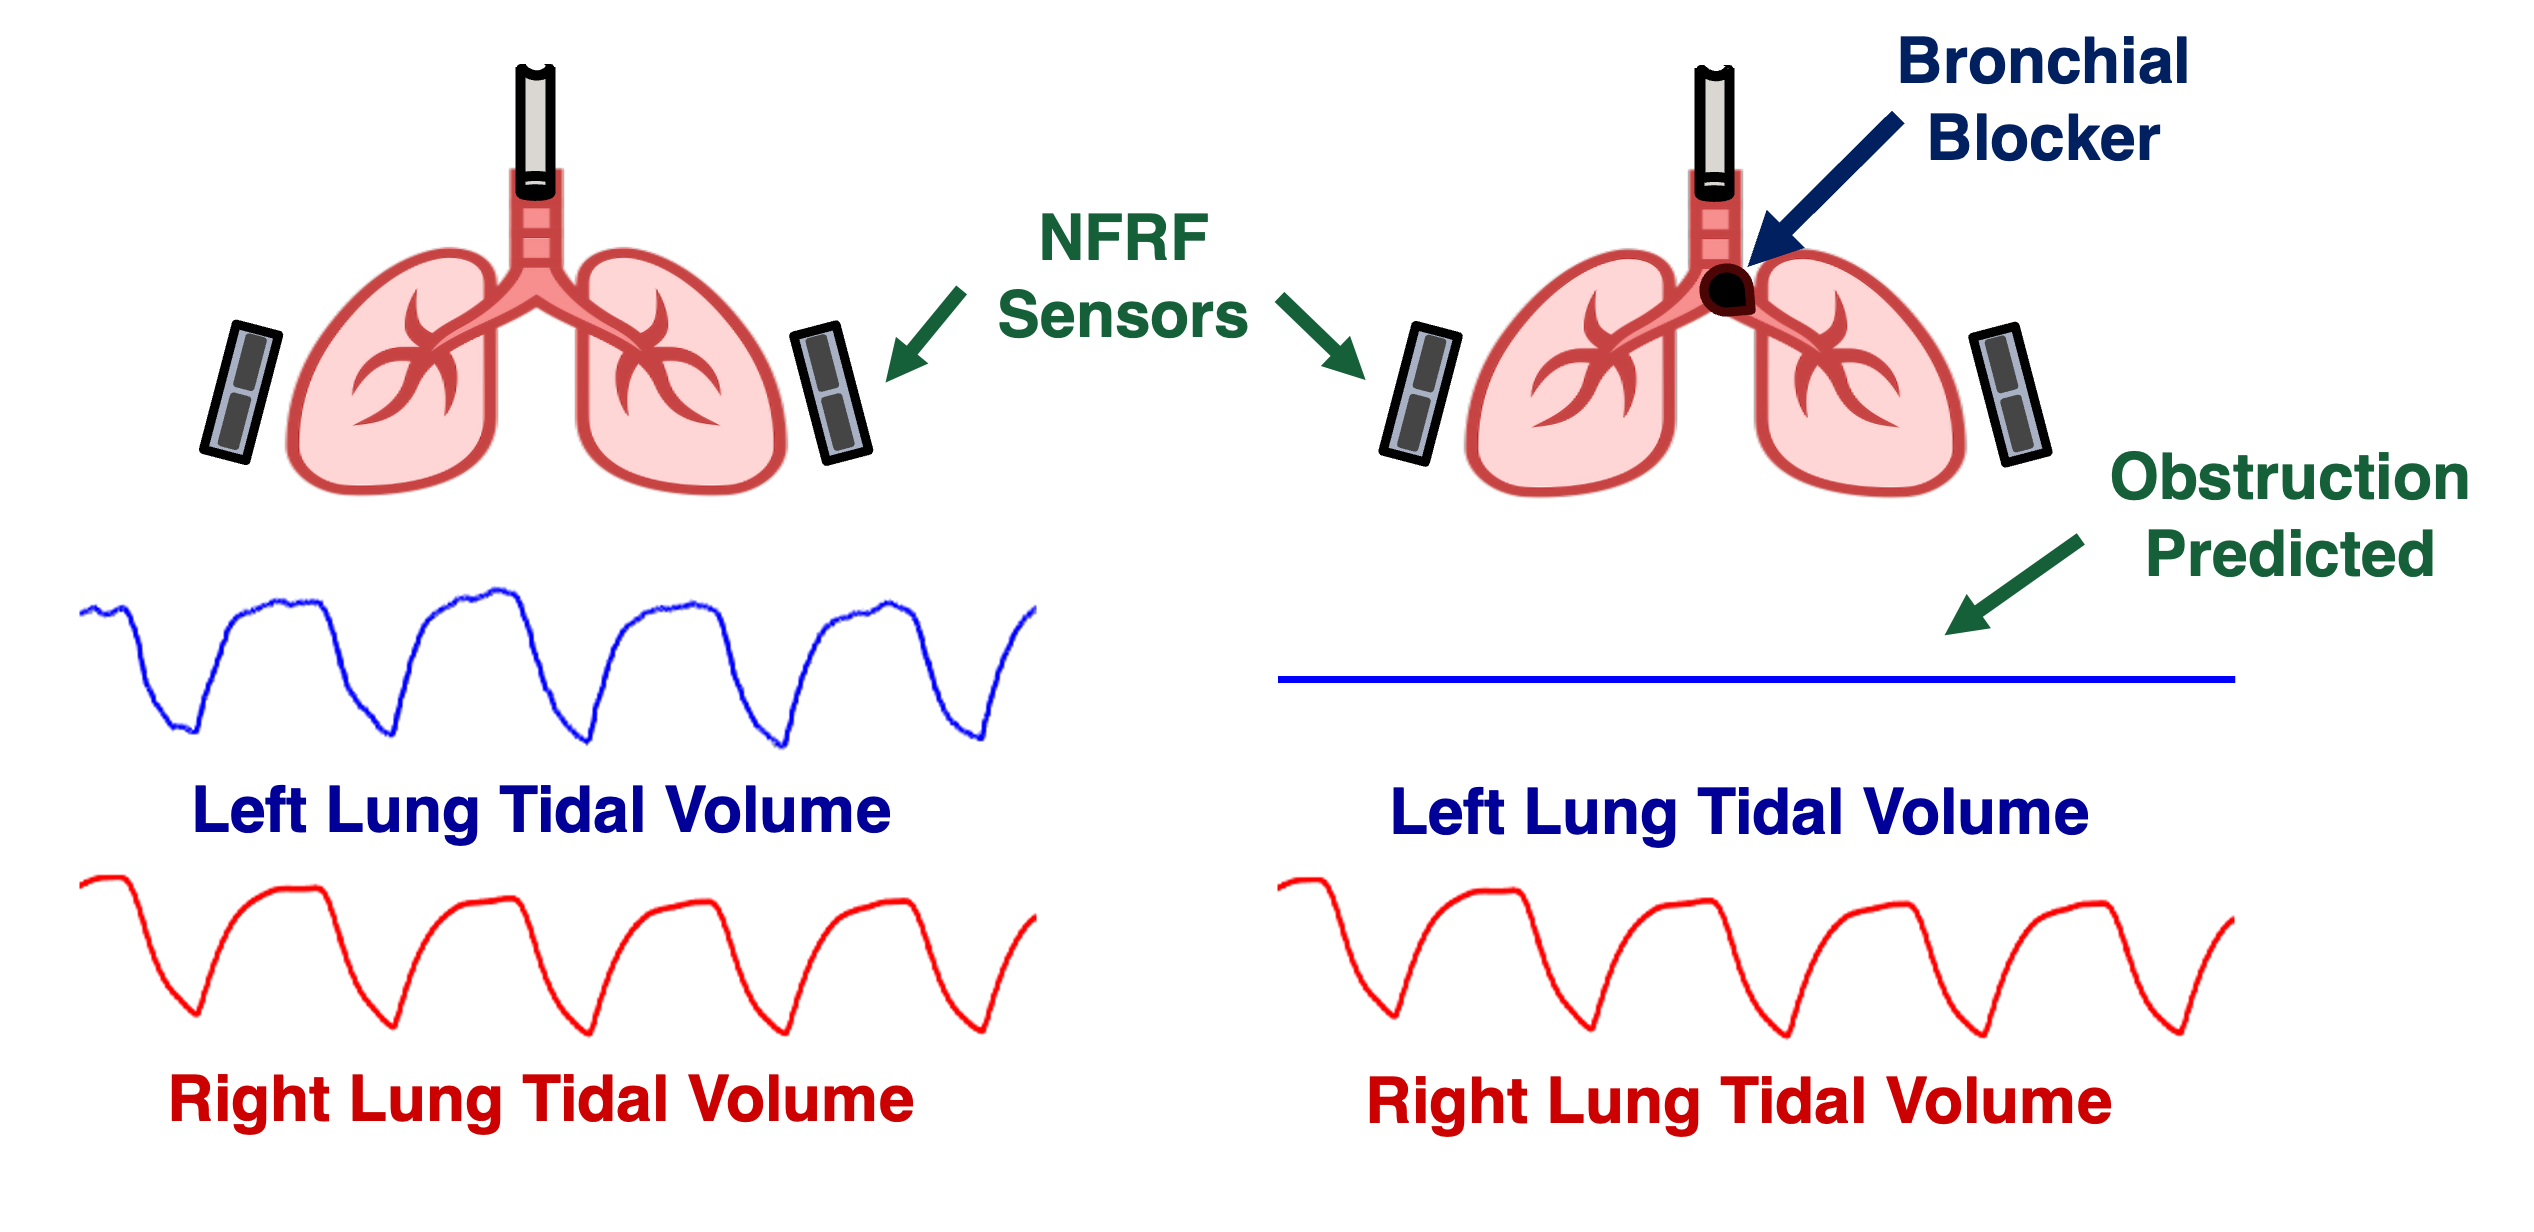
\includegraphics[width=2.96in]{gagraphic3.png}%
\end{wrapfigure}%
\begin{abstract}
Many respiratory disorders are diagnosed by lung function tests, typically performed using spirometers in clinical settings. Non-invasive measures of lung function are of increasing interest to enable convenient, at-home wellness monitoring of respiratory distress. In this work, we used near-field radio-frequency (NFRF) sensors on mechanically ventilated porcine models for continuous acquisition of pulmonary dynamics for each lung independently under various cardiopulmonary interventions. NFRF sensors, previously shown to detect internal tissue motion, were deployed laterally across the pig chest to measure tidal volume during a stepped intervention. A reference spirometer was used for validation. We used bronchial blockers to isolate each lung, allowing us to demonstrate the novel capability of individually monitoring lung volumes. We demonstrated lung volume measurements with an average error of 9.2\% between NFRF and reference spirometry. We also showed individual lung dynamics during one-lung obstruction. The results of this work demonstrates NFRF sensors as a novel wearable method for continuous monitoring of individual lung volumes, aiding the management of respiratory distress during acute and chronic conditions, as well as for detecting early onset of life-threatening conditions such as pneumothorax. 
\end{abstract}

\begin{IEEEkeywords}
Lung volumes, near-field radio-frequency, wearable devices, wellness monitoring
\end{IEEEkeywords}
\end{minipage}}}

\maketitle

\section{Introduction}
\label{sec:introduction}
\IEEEPARstart{P}{ulmonary} health conditions, especially chronic respiratory diseases (CRDs), are among the top causes of mortality globally with some estimates suggesting more than half a billion prevalent cases \cite{viegiGlobalBurdenChronic2020}. Of special concern, two of the most prominent CRDs, chronic obstructive pulmonary disease (COPD) and asthma, exhibit an increasing prevalence among the populace in long-term studies \cite{boersGlobalBurdenChronic2023}. This may be explained by the increasing risk factors for CRDs, including high body-mass index (BMI) and air pollution. Obesity is a major health concern comparable to a hidden epidemic \cite{boutari2022UpdateEpidemiology2022}. Large swathes of the world, primarily under-developed and developing countries, live at unhealthy levels of air pollution \cite{rentschlerGlobalAirPollution2023}. The climate change crisis is expected to exacerbate the situation \cite{andersenClimateChangeRespiratory2023}, under-scoring the urgent need for improving respiratory health monitoring. \\
Increasing global inter-connection due to modern economy and lifestyle has contributed to severe infectious disease outbreaks. Recent pandemics, including severe acute respiratory syndrome (SARS) in 2003, Middle East respiratory syndrome (MERS) in 2012, and COVID-19 in 2019, have involved contagious pathogens impacting respiratory health \cite{bakerInfectiousDiseaseEra2022}. Infectious diseases, trauma, and septic shock are among the leading causal factors for acute respiratory distress syndrome (ARDS). Furthermore, mechanically ventilated patients in intensive care units (ICU) are at particular risks of developing ARDS. Timely management of respiratory conditions is instrumental in improving patient outcomes \cite{leffCOPDClinicalSignificance2005} \cite{arriveEarlyIdentificationDiagnostic2021}, but can be challenging for patients who are less symptomatic or have difficulty communicating their symptoms. \\
Wearable devices contribute to improved health outcomes in multiple ways: providing continuous vital measurements useful for remote health diagnosis, predicting aggravated episodes of chronic conditions, and enhancing integrated disease management. Wearables such as step counters have been observed to improve behavioral patterns which help manage chronic diseases \cite{shahWearableTechnologyInterventions2023}. A meta-review of studies demonstrated the predictability of COPD exacerbation by vital-sign monitoring devices in which lung function measurements using spirometers and blood oxygen saturation levels (SpO$_2$) from pulse oximeters were the most predictive variables of exacerbative episodes \cite{alrajehMonitoringPhysiologicalParameters2016}. \\
\begin{figure*}[htbp]
\centering
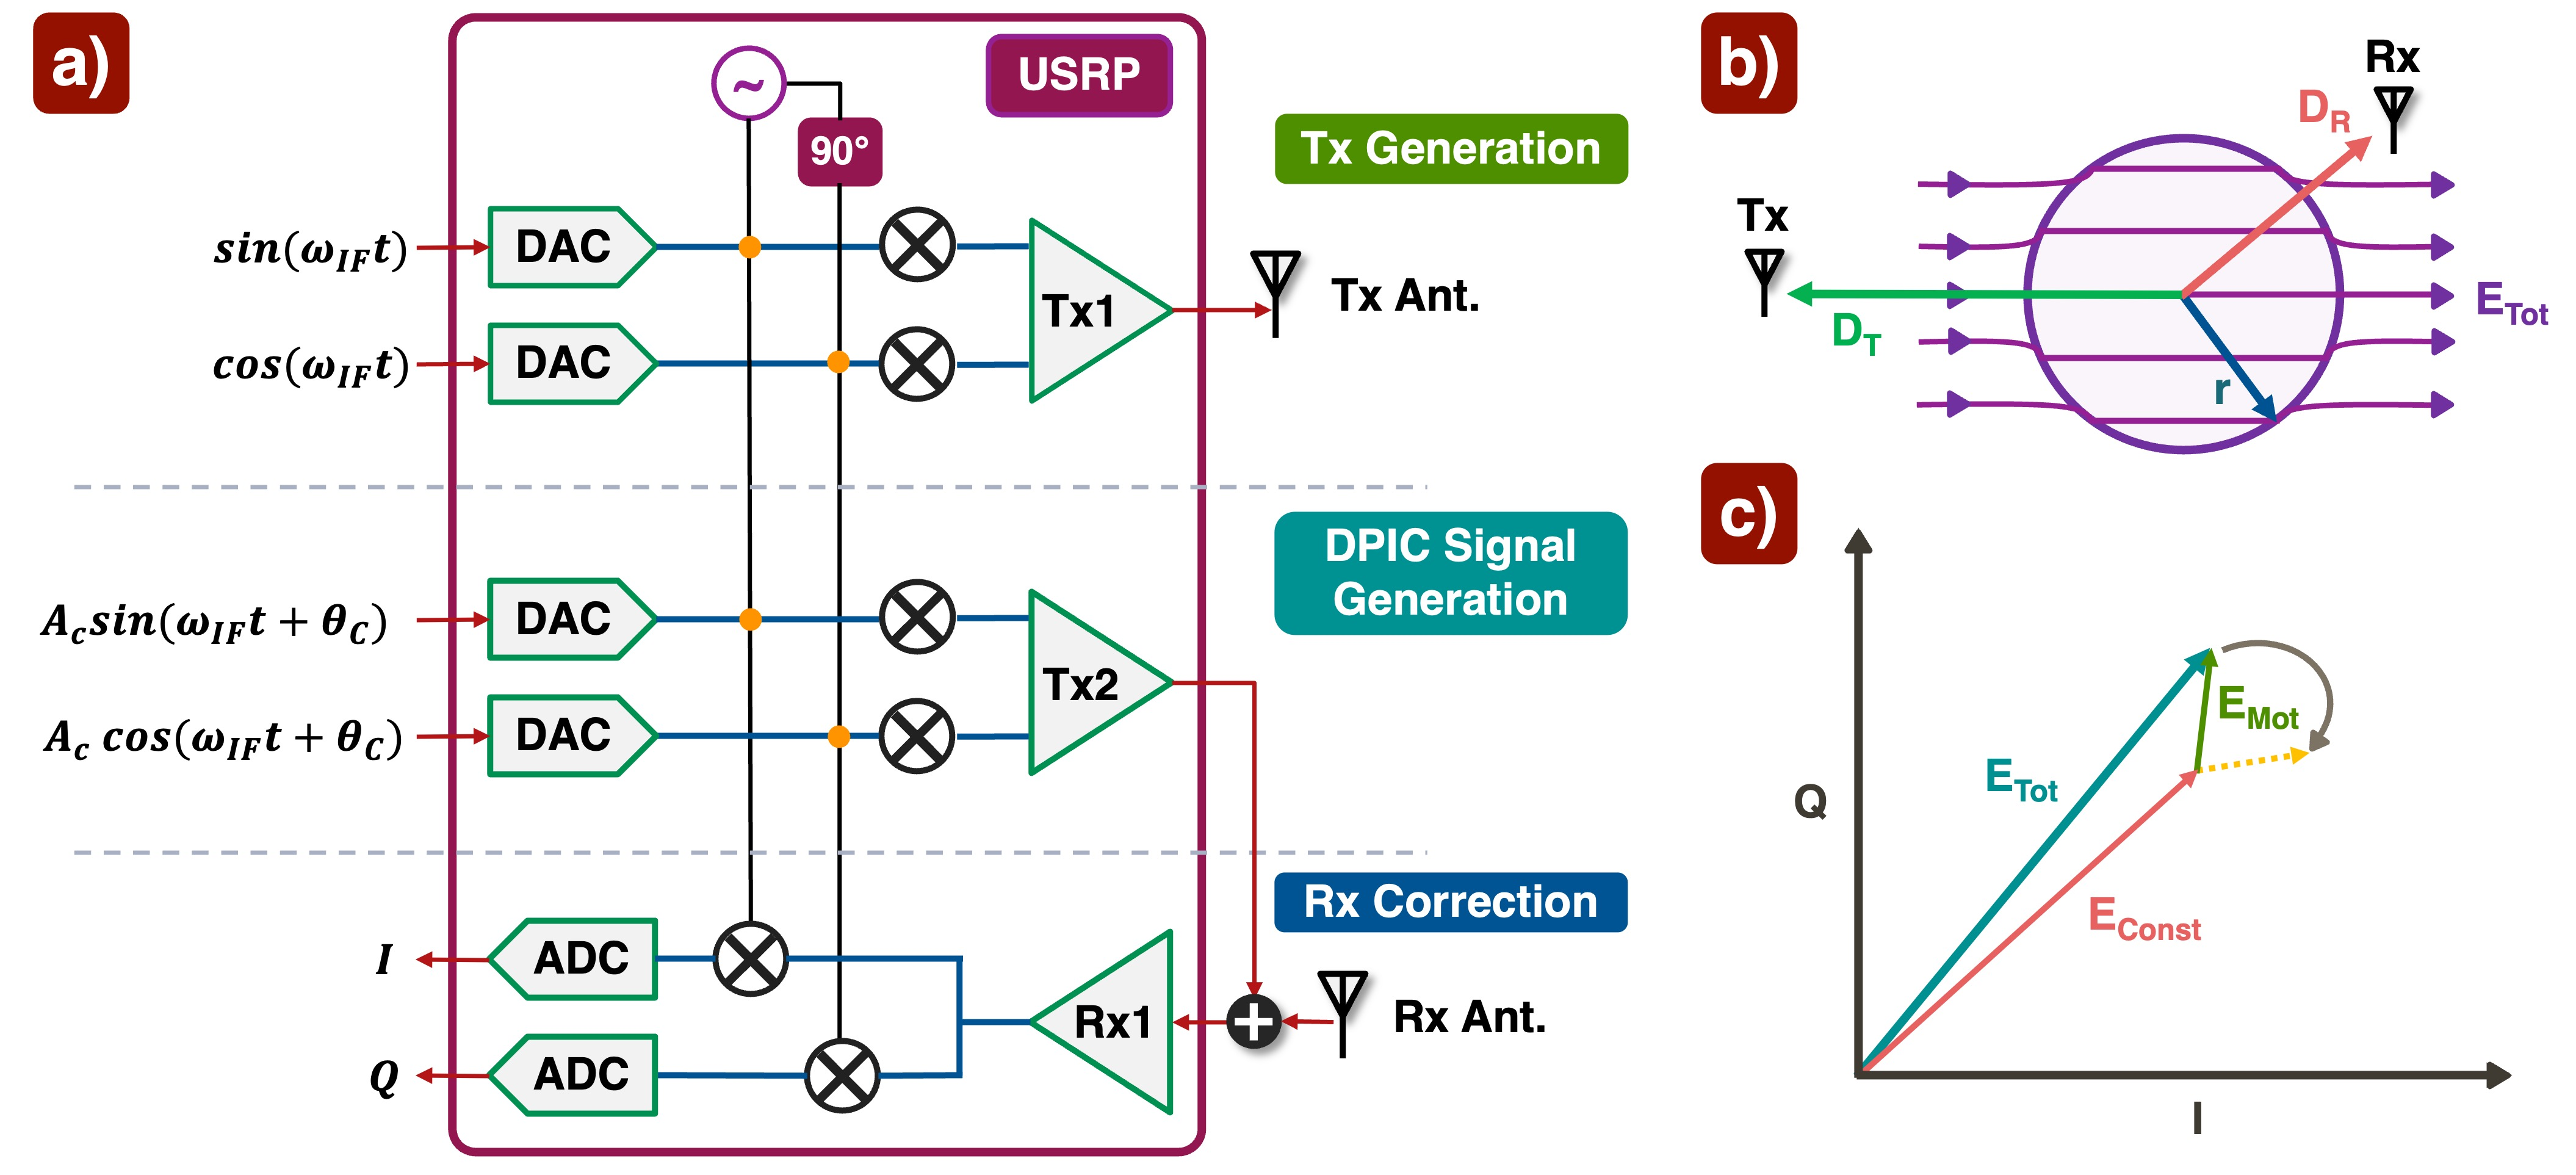
\includegraphics[width=.95\textwidth]{setup_dpic_v3.jpg}
\caption{\textbf{Direct-path interference cancellation in NFRF sensing:} \protect\hl{(a) System schematic; (b) Near-field electric field perturbation by a dielectric sphere; (c) Near-field perturbation electric field showing motion-independent and motion-dependent components}}
\label{fig:dpic}
\end{figure*}
\hspace{-0.5em}Pulse oximeters measure the absorption of light illuminated upon the skin by a pair of light-emitting diodes to derive SpO$_2$ \cite{jubranPulseOximetry2015}. Typically, pulse oximetry is performed at discrete intervals but wearable devices that perform continuous monitoring are widely available as well. SpO$_2$ is a valuable bio-marker indicative of cardiopulmonary health as a whole. However, SpO$_2$ variances may arise from not only respiratory conditions but also cardiovascular issues such as anemia. Further effort is often required to triage low SpO$_2$ levels. Additionally, some studies have observed skin pigmentation biases which may inhibit the general applicability \cite{cabanasSkinPigmentationInfluence2022}. Wearable lung function sensors can augment and further enhance the efficacy of pulse oximeters, enabling more granular diagnosis \cite{buekersWearableFingerPulse2019}\cite{buekersOxygenSaturationMeasurements2018}. \\
Pulmonary function tests measure lung volumes, typically using spirometers as the gold standard \cite{poncePulmonaryFunctionTests2024}. However, spirometers are rarely continuously used due to their inconvenience, bulk, and patient discomfort. Wearable devices capable of estimating respiratory volumes are more suitable candidates for passive and continuous lung function monitoring. While many wearable devices can measure respiratory rates, medical applications require volumetric and gas concentration information. Candidate devices capable of passive and continuous estimation of respiratory volumes include wearable strain sensors \cite{chuRespirationRateVolume2019}, respiratory inductance plethysmography (RIP) \cite{vitazkovaAdvancesRespiratoryMonitoring2024}, and electrical impedance tomography (EIT) \cite{adlerMonitoringChangesLung1997}. \\
RIP is typically performed using two inductive belts placed across the abdomen and chest. The belts contain insulated sinusoidal wire coils. Expansion and contraction of the thorax and abdomen during respiration changes the self-inductance of the coils for resonant frequency measurements, which are proportional to changes in cross-sectional area of the belt, to derive lung volumes. Despite multiple attempts of portable RIP versions \cite{LifeShirtAdvancedSystem}, RIP remains cumbersome due to the system's fundamental requirement of belt tension across both the abdomen and chest. \\ 
Strain sensors use piezoresistivity which exhibits changes in resistance proportional to strain. This allows strain sensors to be significantly smaller and more convenient than RIP devices. Similar to RIP, strain sensors are usually placed across the abdomen and chest, typically by the use of elastic belts, to estimate lung volume dynamics by measuring changes in the chest surface. Piezoresistive strain sensors are versatile and may be integrated into smart clothing. However, they are sensitive to movement artifacts which require additional equipment, such as accelerometers, for correction \cite{defazioOverviewWearablePiezoresistive2021}. Since strain sensors and RIP are limited to measuring changes in the chest surface, they cannot differentiate between individual lung volumes and cannot be used for early detection of abnormalities such as atelectasis. \\
EIT uses electrodes placed around the thorax, with small alternating current (AC) excitation. The resulting voltage measurements are used to reconstruct internal impedance distributions. Suitable parameter reconstruction algorithms are used to generate tomographic images \cite{mansouriElectricalImpedanceTomography2021}. An appropriately large number of electrodes must be chosen for sufficient spatial resolution. This is particularly crucial for EIT images towards estimating lung function \cite{pennatiElectricalImpedanceTomography2023}. EIT systems are non-invasive, real-time and economical in comparison to techniques such as X-ray-based computer tomography (CT). However, image reconstruction from EIT may still be computationally intensive which might be of concern for long-term wearable monitors \cite{boyleAddressingComputationalCost2012} and current available commercial units are expensive and require specialized expertise for application. \\
\sout{Near-field radio-frequency (NFRF) sensing provides a viable alternative to the above vital-sign monitoring technologies. } \hl{Near-field radio-frequency (NFRF) sensing provides a promising alternative to the above methods, without requiring the use of tension belts across the abdomen or skin-touch electrodes, which are uncomfortable and not suitable for long-term wear, especially under heavy perspiration.} Transmitting (Tx) and receiving (Rx) antennas placed proximal to the chests of human study participants were used for sensing tissue motion and tidal volumes were estimated under a variety of conditions using a linear regression model \cite{sharmaWearableRFSensor2019}\cite{sharmaWearableRadiofrequencySensing2020}. NFRF setups have also been attempted for evaluating respiratory efforts in COPD patients and for providing objective respiratory scores to correlate with subjective dyspnea self reports \cite{zhangFeasibilityStudyUsing2024}\cite{zhangObjectiveScoringPhysiologically2022}. The versatility of the NFRF method has been demonstrated by integrating sensors in beds for detection and prediction of sleep apnea \cite{zhangFurnitureIntegratedRespirationSensors2021}.  This paper introduces an NFRF sensor principle for designing an interpretable veterinary study for lung volume characterization. We deployed an NFRF system with enhanced self-interference cancellation upon 8 anesthetized and mechanically ventilated pigs. A stepped tidal volume intervention was examined to validate the ability to track lung volume dynamics across a wide range of lung conditions. Individual lung ventilation was achieved by selective bronchial collapse. The NFRF sensors were able to identify the reduction in ventilation of the collapsed lung which may have applications ranging from detection of acute pathology such as pneumothorax as well as confirmation of adequate lung isolation during surgical thoracoscopic procedures.

\section{Methods}
\subsection{Near-Field Radio-Frequency Sensing}
Dielectric boundary motion, including surface and tissue, in the near-field region of a transmitter (Tx) antenna modulates the antenna characteristics \cite{huiMonitoringVitalSigns2018}, and can be retrieved in the receiver (Rx) baseband in both the magnitude and phase under the quadrature modulation scheme. For a spherical dielectric with time-varying radius in the near-field region of Tx antenna \cite{zhouBackscatterFieldModel2023}, the electric field strength of the continuous wave at Rx can be modeled by the backscattering approximation as:  
\begin{equation}
    E_{tot} = E_{mot} + E_{const}
\end{equation}
where $E_{tot}$ is the total electric field, and $E_{mot}$ and $E_{const}$ are its motion-dependent and motion-invariant components. In the case of a nearly isotropic antenna, $E_{mot}$ takes the form 
\begin{equation}
    E_{mot} = k \frac{r^{3}(t)}{D_{T}^3(t) D_{R}^3(t)} 
    \label{eq:motion}
\end{equation}
where $r(t)$ is the time-varying radius of the dielectric sphere, and $D_T(t)$ and $D_R(t)$ are the distances between the center of the sphere and the phase centers of the Tx and Rx antennas at time $t$, respectively, and $k$ is a proportionality term which depends upon the dielectric properties of the sphere and ambient as shown in Eq.~\ref{eq:prop_const}. For our study, we reasonably assumed that $D_T(t)$ and $D_R(t)$ were time-invariant and $k$ was a constant. 
\begin{equation}
    k \propto \frac{\varepsilon_{sphere} - \varepsilon_{ambient}}{2\varepsilon_{ambient} + \varepsilon_{sphere}}
    \label{eq:prop_const}
\end{equation}
The resultant time-varying electric field is expected to correlate linearly with the dielectric sphere's volume. Eq.~\ref{eq:motion} indicates that the magnitude of the received baseband NFRF signal should be proportional to the total lung volume with the periodic peak-to-peak variations being representative of lung tidal volumes. Although lungs are not spherical, it is still expected that small volumetric changes can be approximated as nearly linear, with nonlinear correction for larger changes in lung volumes. 

\subsection{Direct-Path Interference Cancellation}
Direct-path transmission between Tx and Rx is a strong interference to the desirable signal containing the modulated information from dielectric boundary motion. Direct-path interference (DPI) reduces the effective number of ADC bits for representing baseband information of tissue motion, leading to an increase in the quantization noise \cite{zhouMorphologyTransformationContent2022}\cite{kuoFullyIntegrated60GHz2016}. DPI cancellation, as shown in Fig.~\ref{fig:dpic} becomes crucial, especially because frequencies as low as 0.1 Hz, such as during slowed breathing epochs, can be of potential interest. DPI is sensitive to placement variations in antenna detuning, requiring new setting of DPI cancellation with every significant change to sensing positions and ambient surroundings. DPI is also sensitive to the random initial phase of the transceiver local oscillator (LO) and needs to be reset after the transceiver reboot \cite{xuPhaseOffsetCalibration2024}. While the signal periodicity is not affected by DPI, signal morphology can be deformed, making NFRF signals without DPI cancellation useful mainly for rate-based analysis.
We performed DPI cancellation post suturing the NFRF sensors laterally across the subject chest. Optimal DPI parameters were estimated by performing a parametric search over Tx gains and initial Rx phases so as to restrict the received signal power within optimal ranges of ADC operation \cite{huiNearFieldCoherentSensing2021}.
\begin{figure}[htbp]
\centering
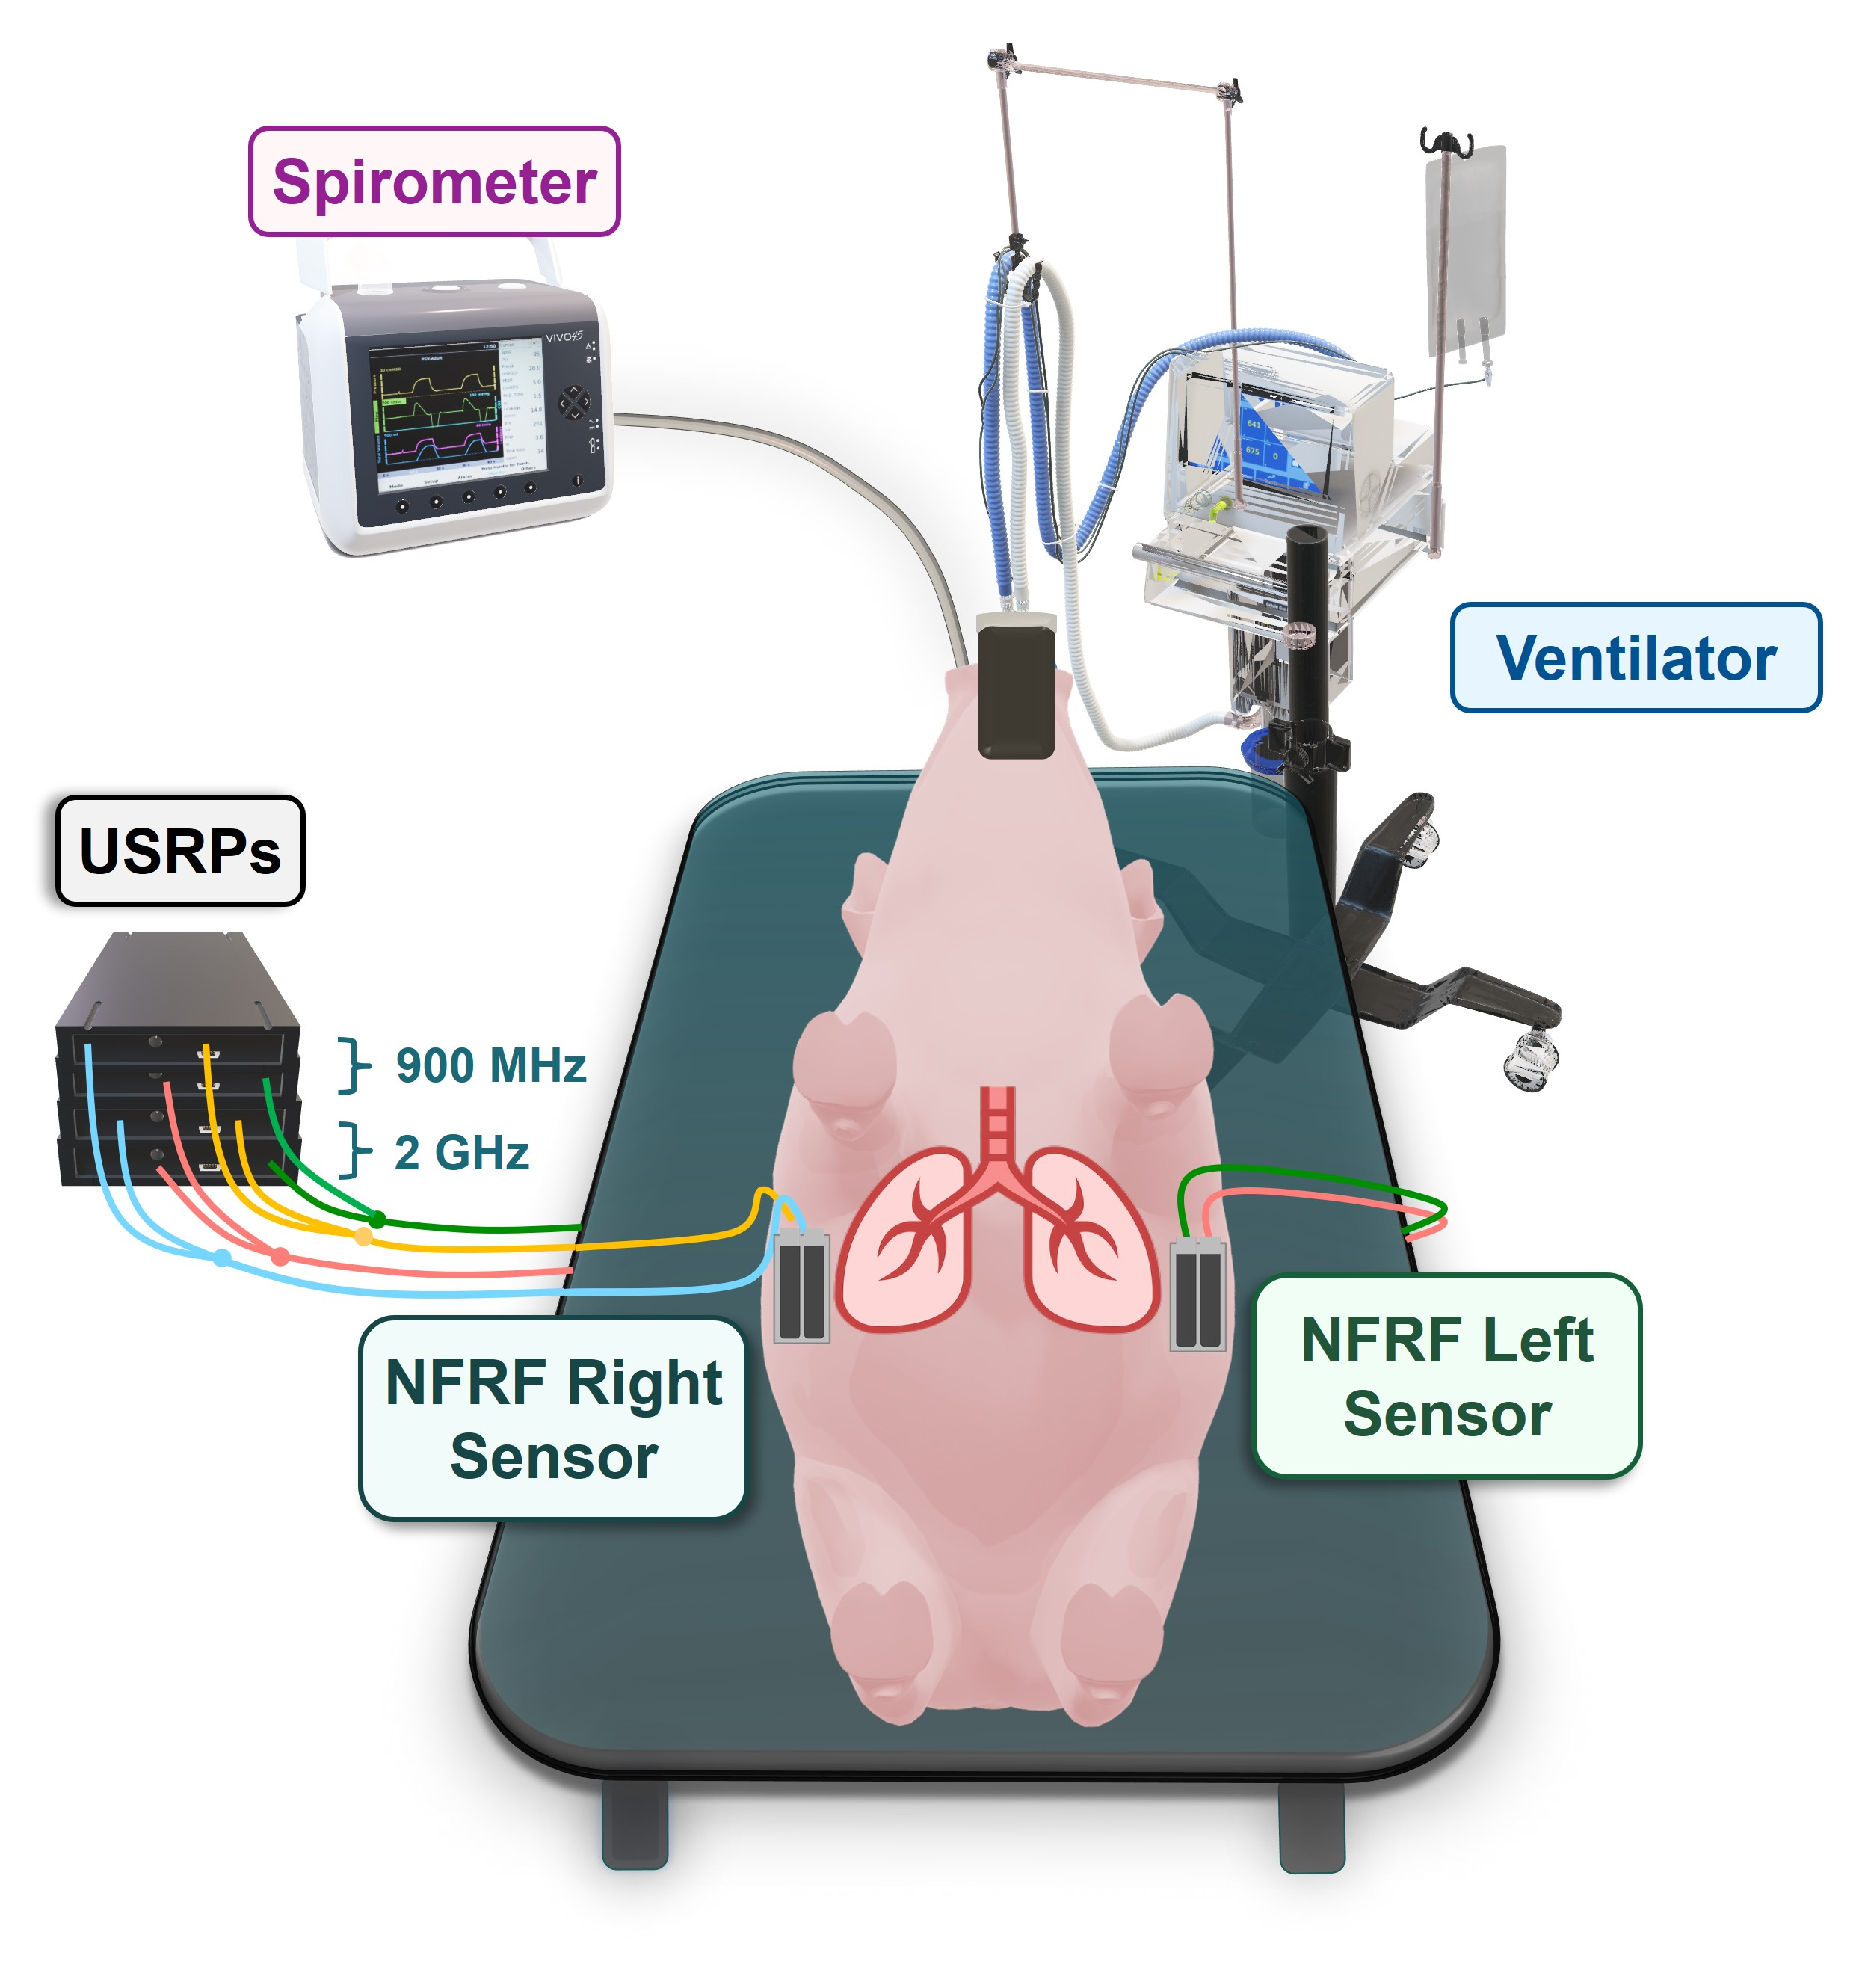
\includegraphics[width=.45\textwidth]{setup_v6.jpg}
\caption{\textbf{Experimental setup:} The NFRF sensing system and reference spirometer were secured upon a mechanically ventilated pig. \protect\hl{Schematics adapted from \cite{pig} \cite{ventilator} \cite{spirometer}.}}
\label{fig:setup}
% Show the ventilator in the figure
\end{figure}
\subsection{Experimental Setup}
Anesthetized and mechanically ventilated pigs were fitted with both the NFRF sensing system and spirometry, as shown in Fig.~\ref{fig:setup}. The procedure was performed under the approved protocols of Cornell University IACUC protocol \#2021-0066 and \#2018-0034. \sout{Spirometer (NM3 monitor; Respironics Inc.) and NFRF sensors were controlled using separate computers, with system time-stamps continuously recorded independently. These time-stamps were subsequently used in post-processing for data synchronization.} \hl{Spirometer (NM3 monitor; Respironics Inc.) and NFRF sensors were controlled using two different computers running ICULab (KleisTEK Advanced Electronic Systems) and a custom LabView (National Instruments Corp.) program, respectively. The two data streams were synchronized by aligning recorded time stamps. A subsequent synchronization validation step was performed by aligning clinical annotations and epochs of ventilatory pauses within a 10 second window, yielding precise data stream alignment to under 0.1s.}\\
Radio signals were generated by means of four National Instruments Ettus Research B210 Universal Software Radio Peripheral (USRP) devices. We employed a dual-frequency band approach, making use of 900 MHz and 2 GHz carriers in order to minimize the impact of potential bi-phasic behavior of received backscatter signal \cite{zhouBackscatterFieldModel2023}. Two pairs of dual-band Pulse W1902 antennas were chosen for sensing. The near-field region, defined within one wavelength, is 33.3 cm and 15 cm in free space for the two carriers, respectively. In lung tissues, these distances reduce to around 10 cm and 4.5 cm. Both carriers were therefore adequate for NFRF sensing but small enough to allow localized capture volume. Selective localization was achieved by placing sensing antenna pairs on laterally opposite sides of the chest, as shown in Fig.~\ref{fig:setup}. This enabled separate measurement of each lung for volumetric estimation. For the present study, we ensured secure fixture by placing Tx and Rx antenna pairs inside 3D-printed casings sutured onto the skin. Alternatively a combination of adhesives and chest belts can also be deployed. The Philips Respironics NM3 spirometer provided measurements of airflow and partial pressure of $O_{2}$ as reference. 
\subsection{Experimental Protocol}
NFRF signals were validated against the reference spirometry by using a step-wise protocol with clinical intervention. The ventilator was set to the volume control mode with the tidal volumes varying from 150 mL to 640 mL in steps of 70 mL, for a total of 8 stages. Each stage was maintained for a period of at least 30 seconds in order to ensure sufficient transient-free data for subsequent analysis. Continuous monitoring of tidal volumes of each lung independently is crucial for diagnosing medical emergencies and surgical procedures. \\
Medical conditions such as atelectasis, where part or all of a lung collapses, can be identified by a reduction in ventilation to the affected region. Emergency situations, such as pneumothorax, often result in uneven ventilation with decreased airflow to the impacted area, making rapid, radiation-free assessment of bilateral ventilation useful. Additionally, during surgical procedures like thoracoscopic surgery, ensuring effective unilateral lung collapse could be aided by confirming the absence of ventilation in the targeted lung. Surgical procedures, such as those involving treatment of diseased lungs, also require isolation between lungs in order to prevent pathogens from contaminating the healthy lung \cite{smithLungIsolationAnesthesia2024}. 
\begin{figure}[htpb]
\centering
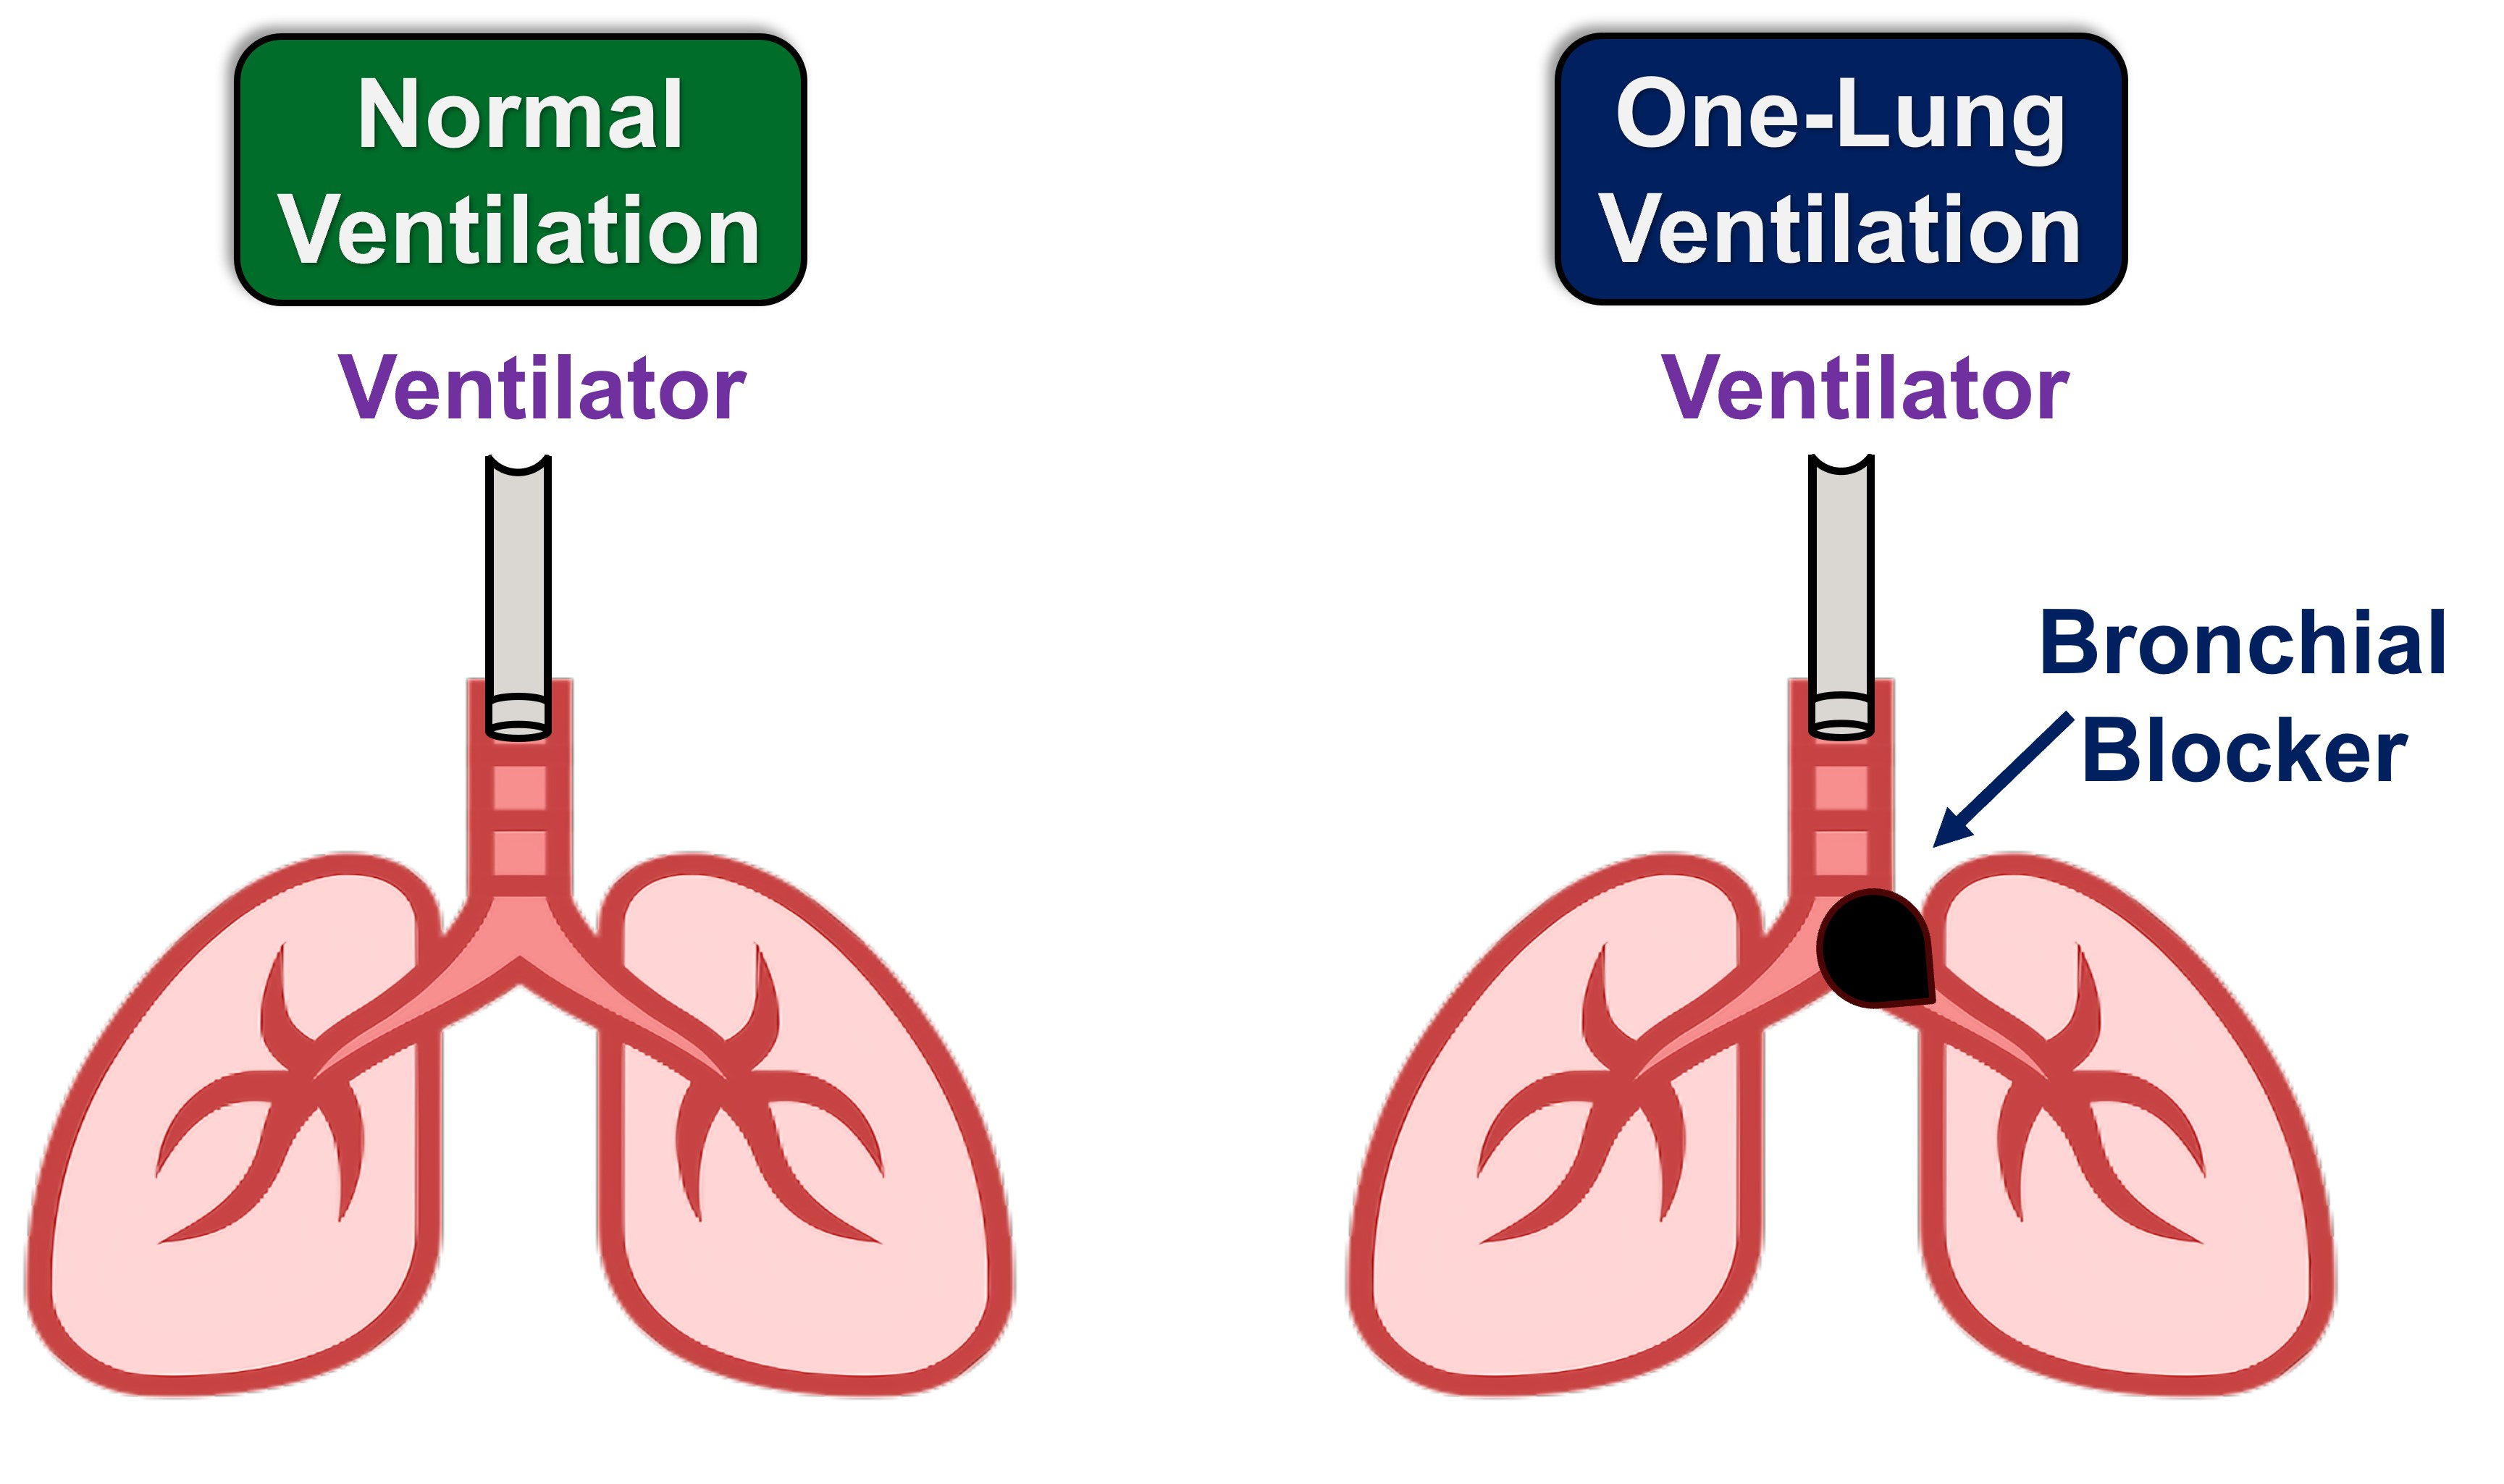
\includegraphics[width=0.48\textwidth]{occlusion.jpg}
\caption{\textbf{Lung obstruction:} Bronchial blockers were introduced into the left main bronchus to induce lung isolation. Lung schematic adapted from \cite{lungImage}.}
\label{fig:occlusion}
\end{figure}\\
Most conventional respiratory sensors, such as wearable strain sensors and RIP which measure chest surface motion, cannot differentiate tidal volumes of each side of the lungs. In comparison, the NFRF system can detect lung isolation induced in mechanically ventilated pigs, as validated by the bronchial blockers, as shown in Fig.~\ref{fig:occlusion}. NFRF signals were continuously recorded while the bronchial blocker was introduced, inflated, and subsequently deflated. The entire procedure spanned a duration of around 15 minutes, including occlusion and post-occlusion recovery. After the test was completed, the ventilator was set on continuous positive airway pressure (CPAP) at 30 cm$H_{2}O$ in order to recruit the previously collapsed regions and reestablish normal lung volumes.  
\section{Signal Processing}
\subsection{Spirometry Reference}
Airway pressure, inspiratory flow, and expiratory flow ($F_A$) were continuously acquired using the spirometer at a sampling rate of 100 Hz. The pressure differential connector of the spirometer was connected between the endotracheal tube and the y-piece of the breathing circuit. The spirometer was calibrated daily using a 3L calibrated syringe (Hans Rudolph). High-frequency noises such as the line noise and DC shifts in the integrated airflow were properly bandpass-filtered between 0.05 Hz and 15 Hz for a consistent tidal volume reference. Filtered airflow was numerically integrated using trapezoidal integration to obtain continuous-time tidal volume reference $V^{spiro}_T$. 

\subsection{Fiducial Point Extraction} \label{sec:fiducial}
Airflow for mechanical ventilation followed a standard morphology along with key fiducial points, as shown in Fig.~\ref{fig:airflow}. Fiducial points were extracted from filtered airflow waveforms to segment individual breaths, using the steps below. 
\begin{itemize}
    \item \textbf{Breath rate estimation:} Fourier transform of airflow data was computed. The highest peak, corresponding to the principal breath rate, was used to extract the initial breathing rate $\hat{r}_{br}$. This yielded an average breathing duration $\hat{t}_{br} = 1/\hat{r}_{br}$
    \item \textbf{Airflow processing:} Filtered airflow data were differentiated along time to obtain $d_{flow}(t)$ 
    \item \textbf{Inspiratory and expiratory flow starts:} Maxima and minima in $d_{flow}(t)$, separated by $\hat{t}_{br} \times f_{s}$ samples, were extracted using \texttt{findpeaks} in Matlab to obtain the inspiratory and expiratory flow starting points. 
\end{itemize}
\begin{figure}[htpb]
    \centering
    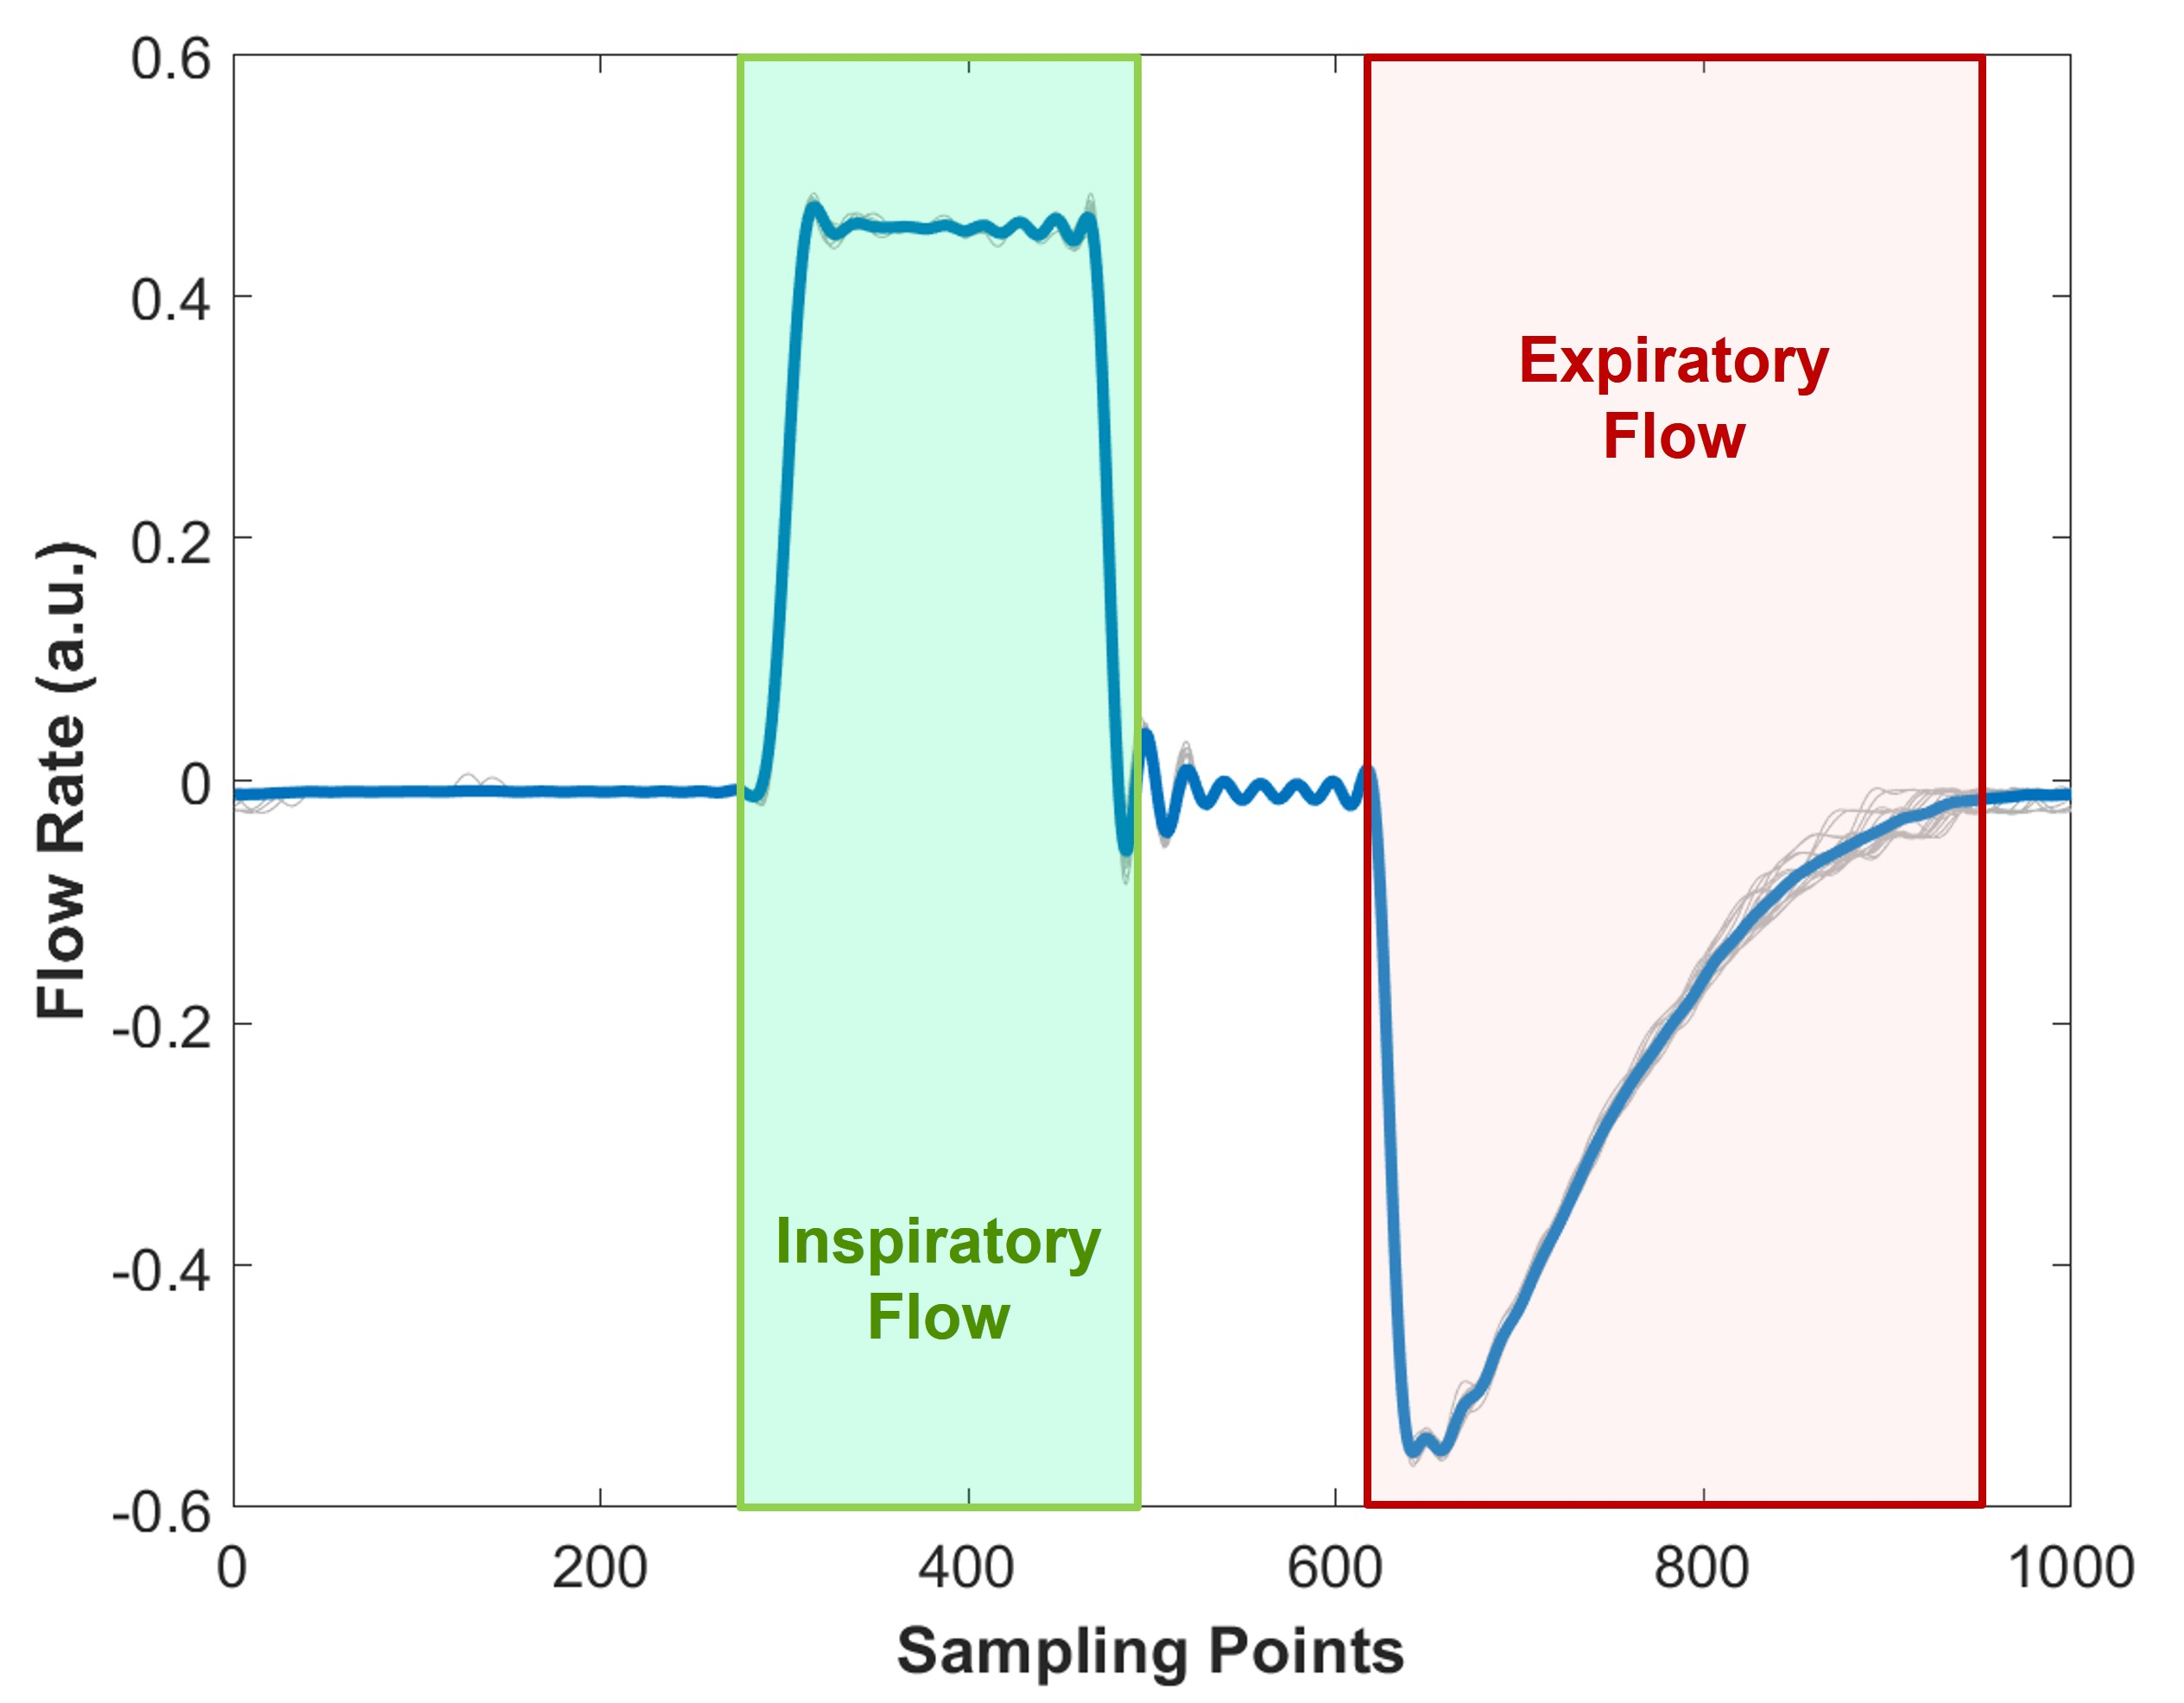
\includegraphics[width=0.5\textwidth]{airflow.jpg}
    \caption{\textbf{Airflow measurement:} Ventilated airflow measured by spirometer shows characteristic differences in inspiratory flow and expiratory flow epochs.}
    \label{fig:airflow}
\end{figure}
Selecting peaks successively separated by $\hat{t}_{br}$ was crucial to avoid detecting false peaks, for example, during a particularly sharp exhalation. The algorithm robustness was enhanced by constraining inspiratory and expiratory flow time points to alternate. This was especially relevant for our study since acquired data contained epochs where airflow had been paused for clinical reasons. The use of the Fourier transform, while valid in our study owing to the use of a fixed breathing rate in the mechanical ventilator, does not necessarily generalize to practical conditions. Situations involving variable breathing rates should employ Short-Term Fourier Transform (STFT) over appropriately chosen sliding window lengths.

\subsection{NFRF Sensors}
The NFRF sensing system acquired quadrature modulated data at a sampling rate of 10 kHz from USRP, which was down-sampled to 1 kHz for storage efficiency. Using Eq.~\ref{ref:iq_to_sig}, we reconstructed signal amplitude and phase, which resulted in 8 channels of data, comprising amplitude and phase at dual carrier frequencies of 900 MHz and 2 GHz per lung. 
\begin{equation}
    \begin{split}
        A(t) &= \sqrt{I^2(t) + Q^2(t)} \\
        \theta (t) &= \text{unwrap}(\arctan \frac{Q(t)}{I(t)})
    \end{split}
    \label{ref:iq_to_sig}    
\end{equation}
For each channel, the down-sampled signal $s_{i}(t)$ was further filtered to reduce random noise, DC shifts, line noise, and motion artifacts. 
\begin{itemize}
    \item \textbf{Spike removal:} Sudden small signal spikes in $s_{i}(t)$ were removed by median filtering, in which each sample value was replaced by the median of samples in a sliding window. After filling in signal gaps with median values, $s_{i}^{(med)}(t)$ was free of ill-defined null values. 
    \item \textbf{Motion artifact removal:} Motion artifacts were often presented as large spikes in the NFRF signal. While they were ameliorated by median filtering, we still observed residual motion artifacts in $s_{i}^{(med)}(t)$. Residual motion artifacts were further reduced by replacing outliers in the NFRF differential signal of $d(t)$ with nearest non-outlier values. The modified $d_{c}(t)$ was re-integrated to obtain motion-corrected signal $s_{c}(t)$.
    \item \textbf{Bandpass filtering:} The motion-corrected signal $s_{c}(t)$ was band-pass filtered between 0.05 Hz and 15 Hz, removing DC trends and line noise, to obtain the filtered signal $s_f (t)$. An advantage of placing the NFRF sensors laterally across the chest is a strong isolation from interference caused by heart dynamics. Without isolation caused from sensor location, frequency components pertaining to heart motion need to be removed using notch filtering to improve peak detection in flow fiducial points. 
    \item \textbf{Segmentation:} Fiducial points of the respiratory waveform, extracted in Sec. \ref{sec:fiducial}, were used to segment $s_f (t)$ for characteristics of each breath.   
    \item \textbf{Multi-breath averaging:} Physiological information capture by the NFRF signals can be made more accurate by averaging over multiple breath intervals \cite{conroyHeartIDBiometric2023}. The number of periods used for averaging was empirically chosen to be 5 which provided a good balance of increased accuracy without violating stationarity or adding a large lag for estimation. 
    \item \textbf{Interpolation:} Per-breath segments were cubic-spline interpolated to a fixed length and averages of 5-breath windows were stored in an array $\{s_f (t)\}_{i=1}^{n}$ for further analysis.
\end{itemize} 
\subsection{Tidal Volume Estimation}
\begin{figure}[htbp]
    \centering
    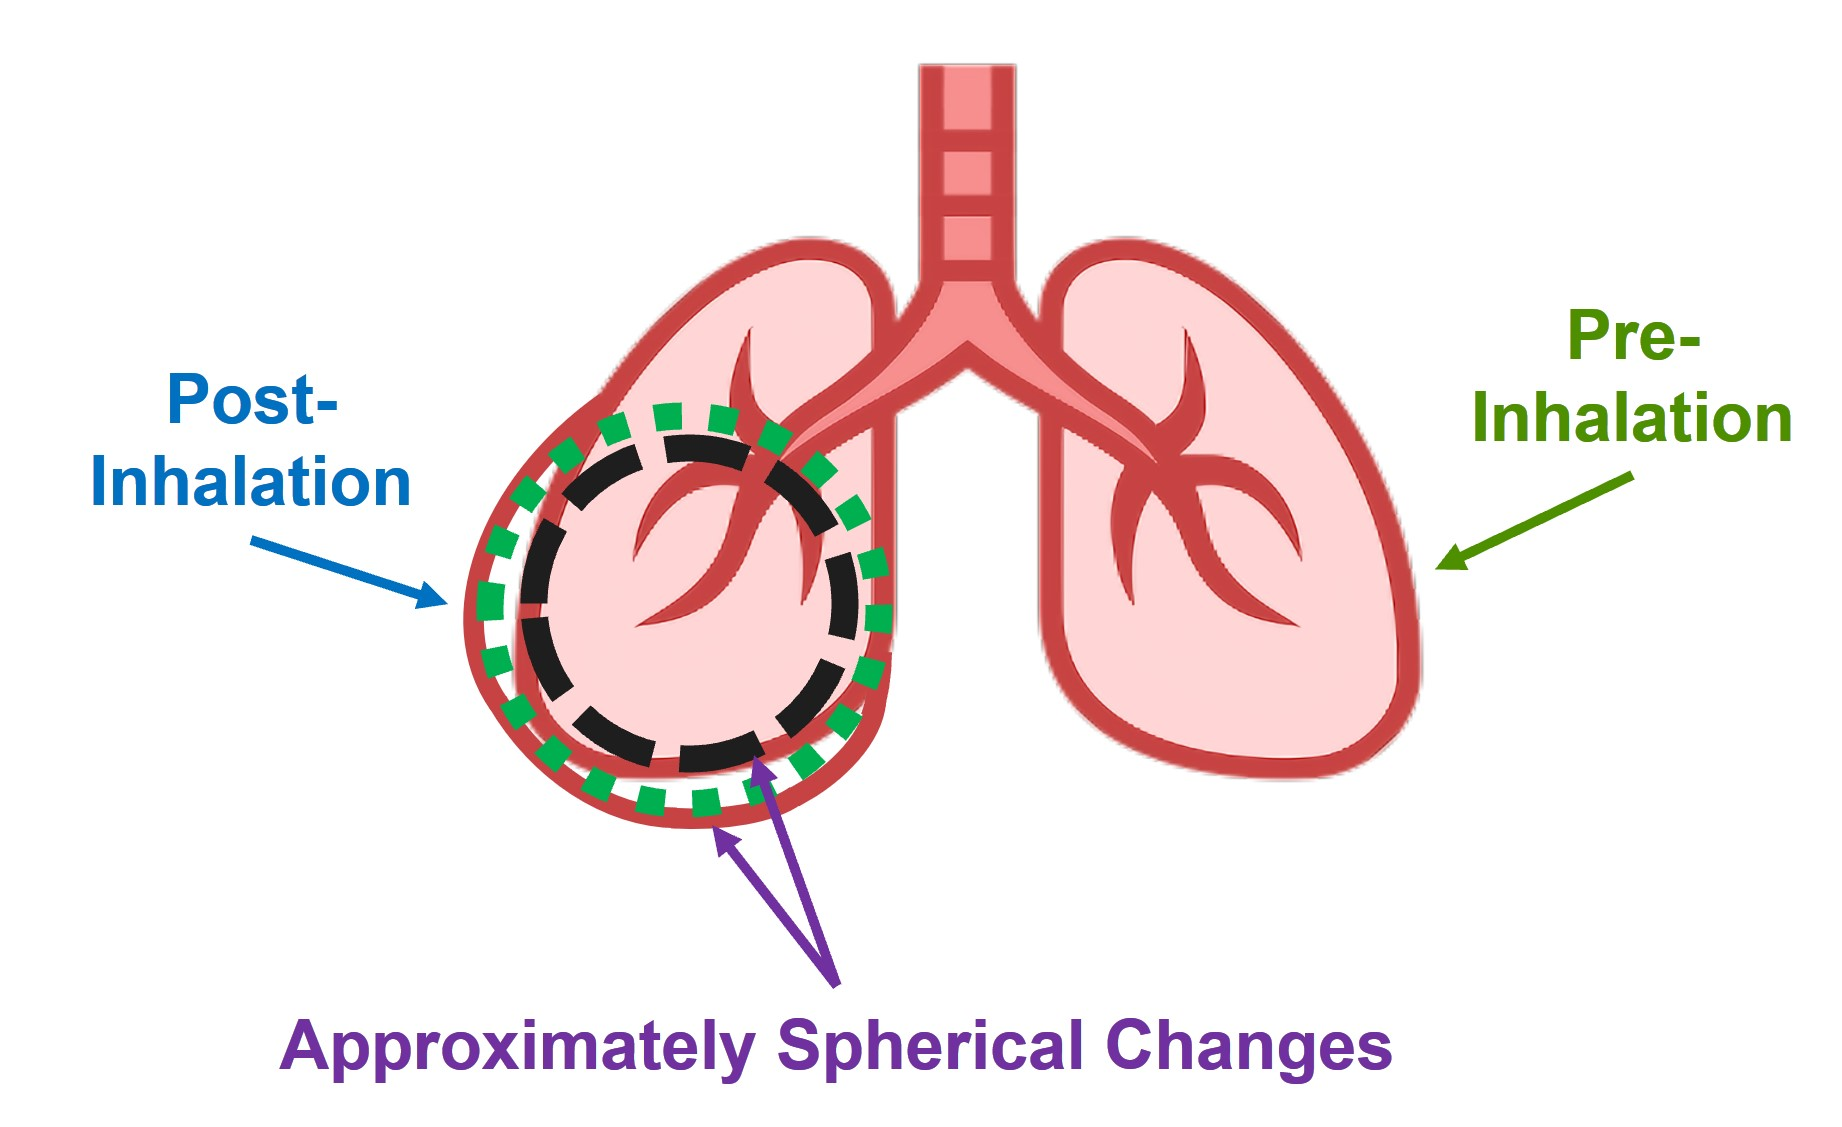
\includegraphics[width=0.5\textwidth]{approx_sphere_v2.jpg}
    \caption{\textbf{Spherical approximation schematic:} Small changes in lung volume corresponding to the regular ranges of tidal volume can be approximated as a nearly spherical body change. Lung schematic adapted from \cite{lungImage}.}
    \label{fig:approx_sphere}
\end{figure}
NFRF sensors capture dielectric boundary motion and Eq.~\ref{eq:motion} suggests a linear correlation between the signal magnitude and lung volume. Small motion in non-spherical dielectrics may be approximated to primarily be the motion of an appropriately chosen spherical subset of the total volume, as shown in Fig.~\ref{fig:approx_sphere}. This chosen spherical subset, exhibiting a majority of the maximal motion, was considered as the main observation. The above sphericity assumption holds for changes in volume much smaller than the maximum lung volume and can be sufficient for tidal volume estimation. The remainder of the tissue is assumed to primarily contribute to the dielectric ambient, impacting $E_{const}$ but not $E_{mot}$. The above assumptions yield Eq.~\ref{eq:lin_vol}, where the measured NFRF signal for the $i$-th channel directly represents the volume of the spherical tissue subset $V_{sub}$ scaled by a channel specific constant $k_i$. 
\begin{equation}
    s_f^{i}(t) = k_{i} V_{sub}(t)
    \label{eq:lin_vol}
\end{equation}
\begin{figure}[h]
\centering
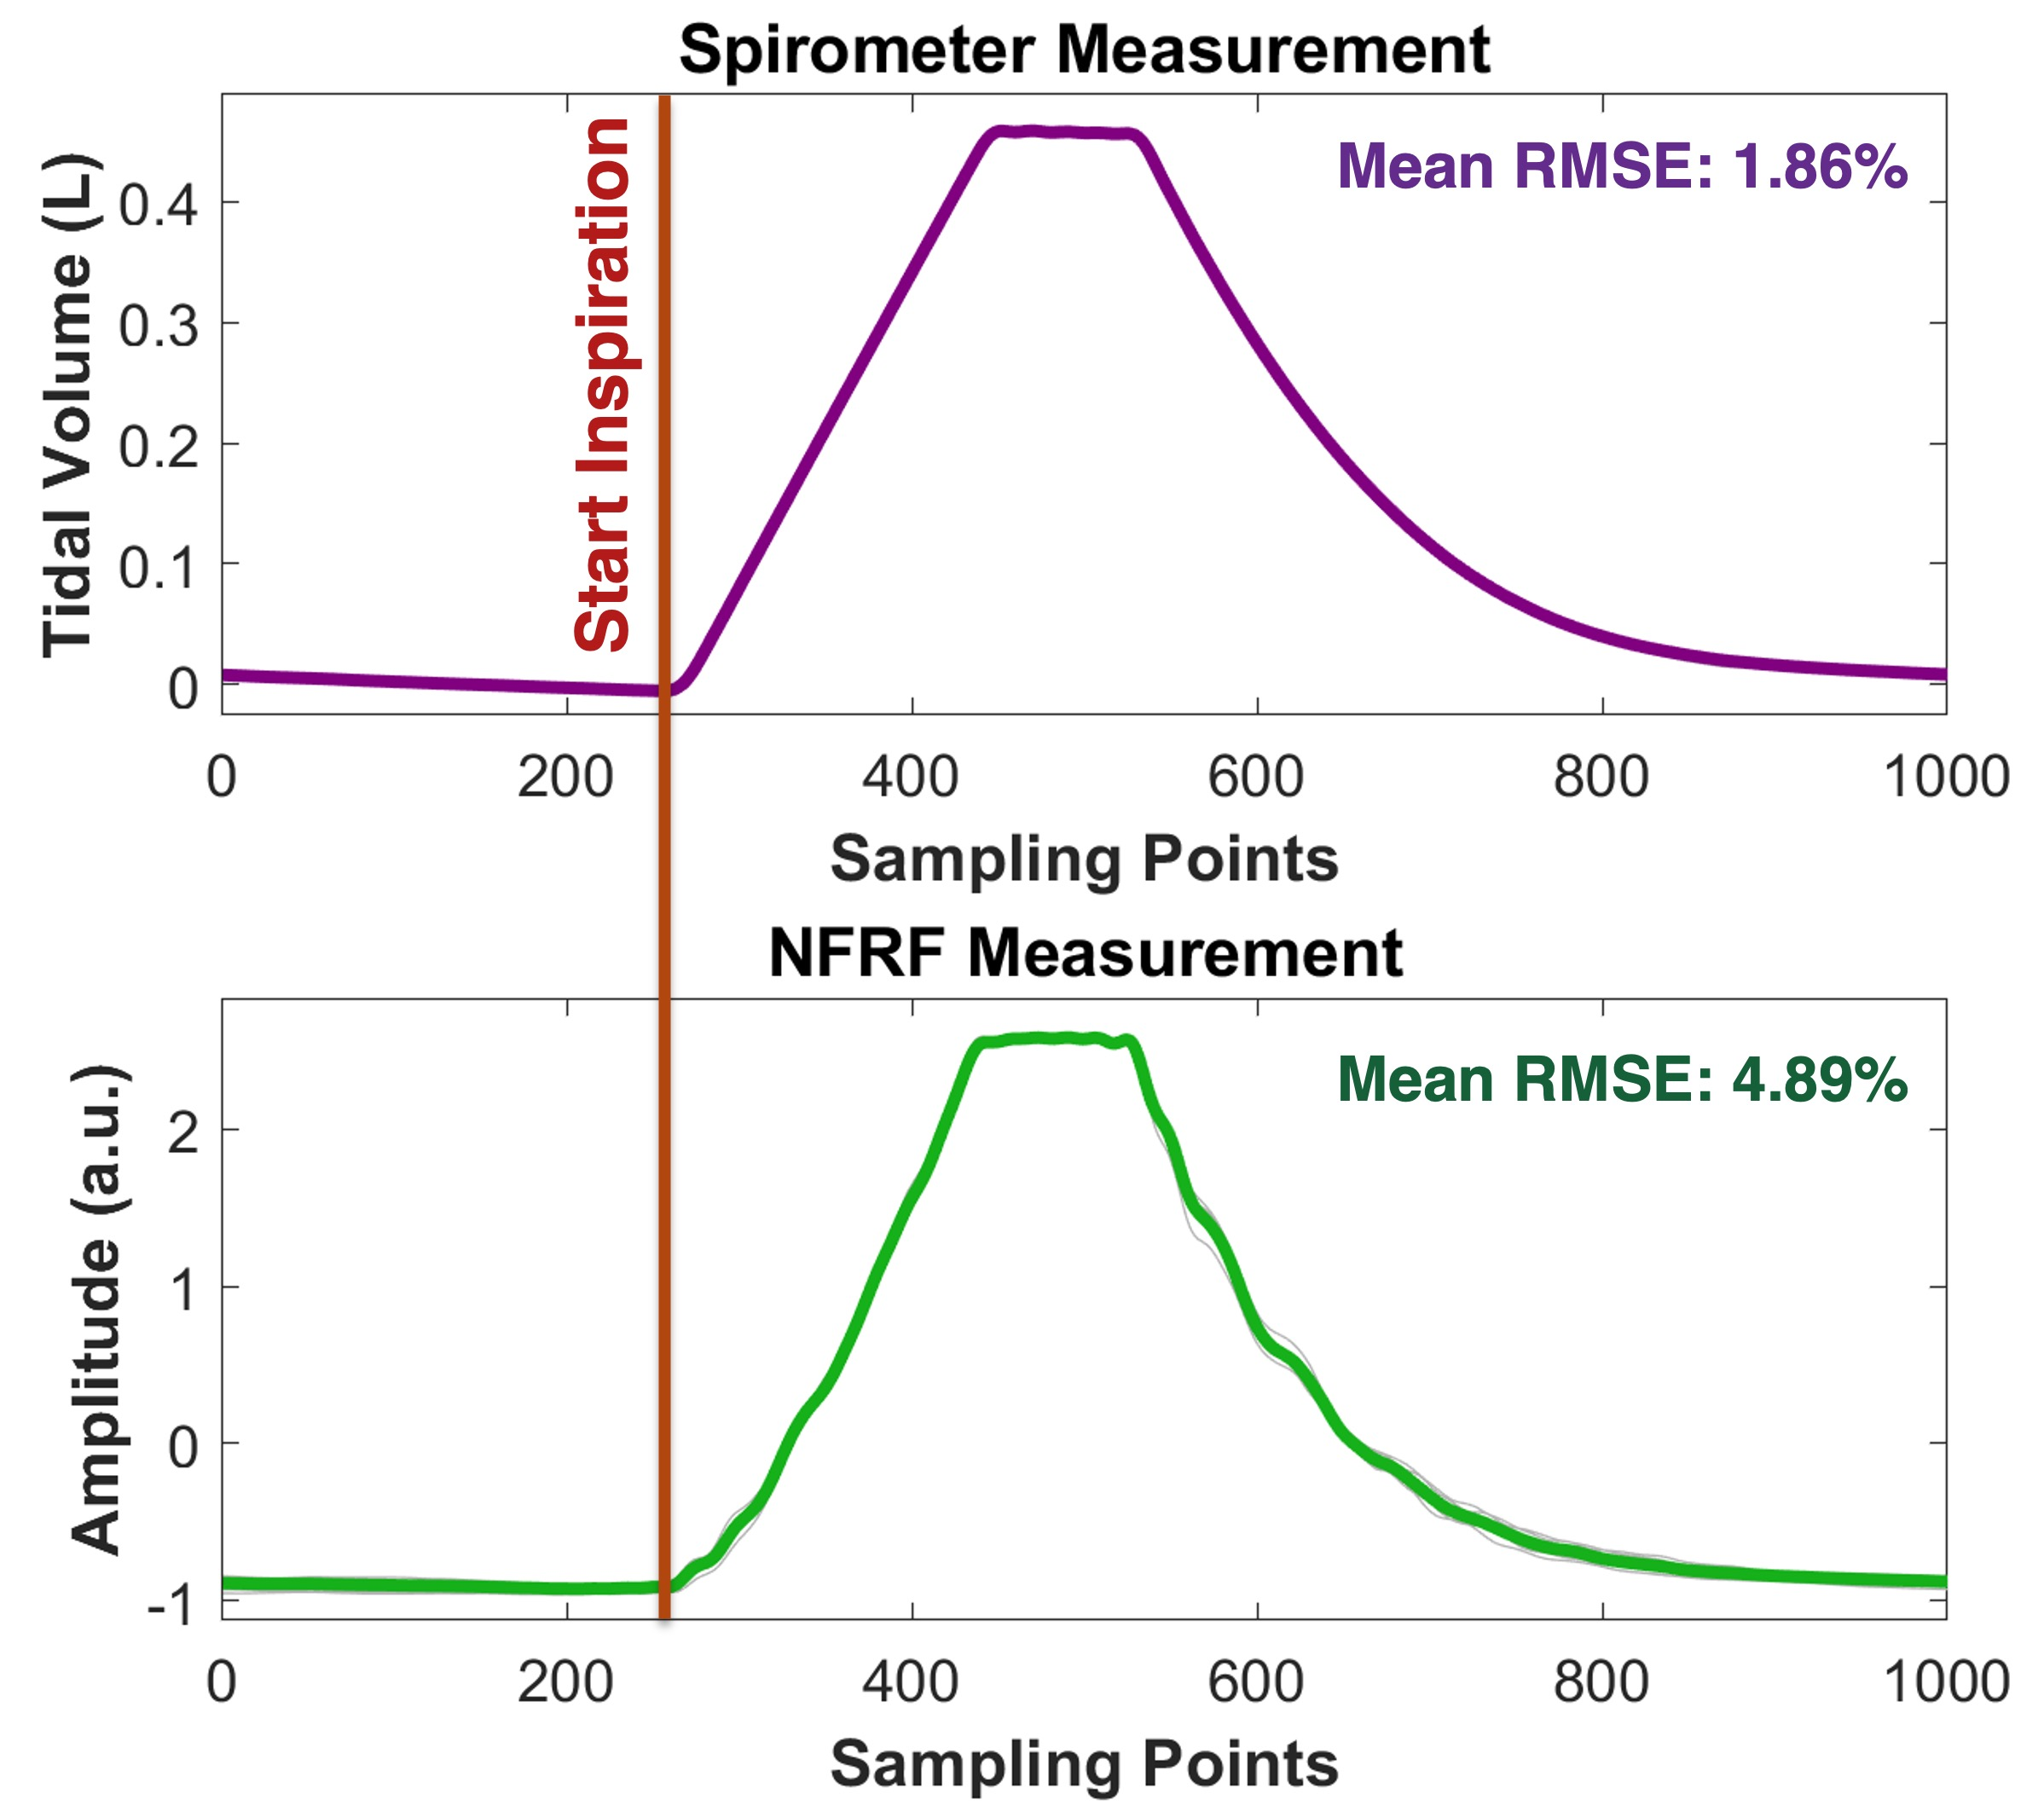
\includegraphics[width=.48\textwidth]{ncs_spiro2.jpg}
\caption{\textbf{Time-domain signal visualization:} Synchronized NFRF and Spirometry signals were segmented, and an average signal template was generated by overlaying 5 consecutive breaths, showing an average RMSE of 1.86\% and 4.89\% among the individual breaths and the average signal template respectively.}
% Is the bold line done by DTW templates?  If so, we should mention that explicitly. 
\label{fig:ncs_spiro_time}
\end{figure}
\\Visualization of the warped signal $s_f (t)$ with synchronized reference spirometry, as in Fig.~\ref{fig:ncs_spiro_time}, underscores the motivation behind this approach. Variations in $V_{sub}$ form the greatest percentage of the lung tidal volume $V_{T}$, given by Eq.~\ref{eq:sub_to_tv}. 
\begin{equation}
    PP(V_{sub} (t)) = g V_{T} (t)
    \label{eq:sub_to_tv}
\end{equation}
where $PP$ represents the peak-to-peak value of input and $g$ is a scaling constant, which may depend upon the specific lung structure of the subject. Peak-to-peak values of the NFRF signals involve the channel scaling constants from Eq.~\ref{eq:lin_vol} and are combined in Eq.~\ref{eq:estimator} below. 
\begin{equation}
    \hat{V}^{i}_{T} = \frac{1}{g k_i} PP(s_f^{i} (t))
    \label{eq:estimator}
\end{equation}
Statistically relevant estimates for scaling constants, both $g$ and $k_{i}$, could be numerically derived by detailed simulations and anatomically accurate physical models. However, these strategies are computationally intensive and incur significant expenditure. It is much easier to empirically obtain the scaling terms by calibrating against a known ground truth. We used reference spirometry to calculate channel-specific calibration constants $c_{i}$, as shown in Eq.~\ref{eq:calibration}, over a short calibration epoch of $t_{cal}$ of 30 seconds at the start of the intervention. 
\begin{equation}
        c_{i} = \frac{V^{spiro}_{T}(t_{cal})}{PP(s_f^{i} (t_{cal}))} 
    \label{eq:calibration}
\end{equation}
where $c_{i}$ are measured estimators for the $\frac{1}{gk_i}$ term in Eq.~\ref{eq:estimator}. Once the sensing system was secured in place and calibrated, it did not need re-calibration until it was perturbed significantly. Thus, empirically derived calibration constants $c_i$ were used for tidal volume estimation throughout the entire duration of the study. Each NFRF channel yields a tidal volume estimate for a total of 8 estimated values.
\begin{equation}
    \hat{V}^{i}_{T} = c_{i} PP(s_f^{i} (t))
    \label{eq:compute_tv}
\end{equation}
NFRF channels exhibited a varying level of signal quality throughout the experiment. Typically, each subject tended to have a set of optimal channels which may not be the same for another subject. Variations in signal quality arose from multiple factors: sensor placement, motion of sensors during data acquisition, and changes of ambient surroundings. Obtaining a high-quality unbiased $V_T$ estimate necessitates combining per-channel estimates using easily quantifiable metrics. The aforementioned variations primarily presented as variations in the signal-to-interference ratio (SIR), defined as the ratio of fundamental breath signal to the median noise between 0.05 Hz and 0.35 Hz, and linearity, computed as the ratio of the fundamental to the second harmonic, of the acquired signal. SIR and linearity were thus used as quality metrics $Q^{i}_{SIR}$ and $Q^{i}_{Lin}$, respectively. Per-channel tidal volume estimates, weighted by normalized quality metrics, are used to compute the overall NFRF tidal volume estimate $\hat{V}^{NFRF}_{T}$ 
\begin{equation}
    \hat{V}^{NFRF}_{T} = \frac{\sum_{i=1}^{n} Q^{i} \hat{V}^{i}_{T}}{\sum_{i=1}^{n} Q^{i}}
    \label{eq:combine_channels}
\end{equation}
Redundant channels are a key advantage of NFRF as they can make the system more robust in comparison to sensing systems which only have one measurement channel. For our analysis, we decided to sort channels based on their initial quality estimates and discard the bottom-half for estimates. This provided an increase in robustness for our system as each pig had a different ambient and body in sensor arrangement. 

% \subsection{Flow Extraction}

\section{Results}
\subsection{Continuous Tidal Volume Estimation} \label{sec: tidal_vol_estimation}
\begin{figure*}[t]
\centering
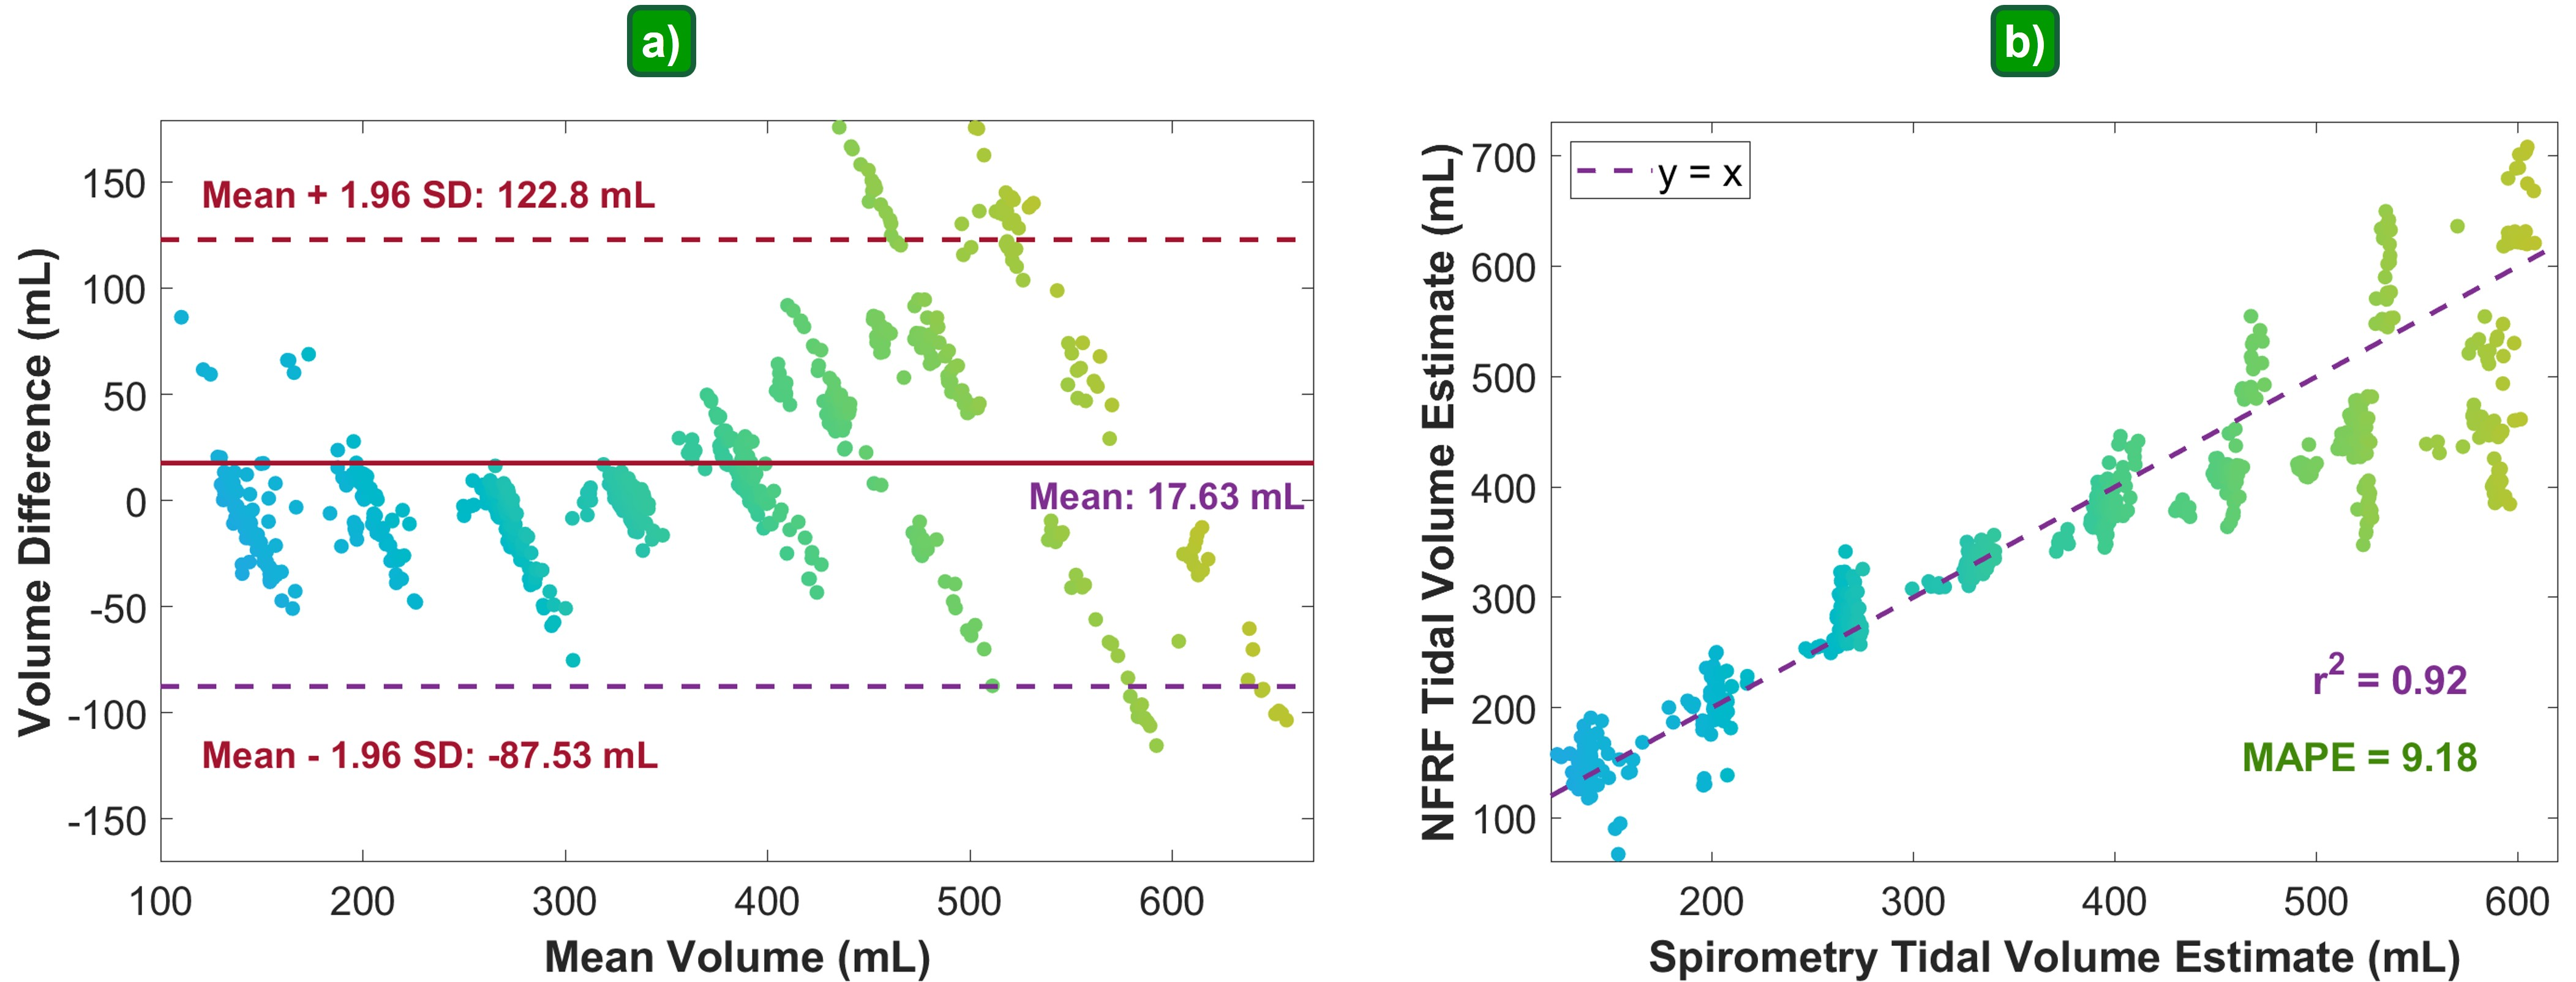
\includegraphics[width=.98\textwidth]{results_v3.jpg}
\caption{\textbf{NFRF system characterization:} (a) The Bland-Altman plot; (b) Correlation plot for data acquired over all subjects throughout the study}
\label{fig:results}
\end{figure*}
\sout{Bland-Altman (B\&A) plots \cite{martinblandSTATISTICALMETHODSASSESSING1986}\cite{blandComparingMethodsMeasurement1995} are a well-accepted method for comparing two clinical measurements, typically to quantify the performance of a technique against an existing gold standard.} \hl{Bland-Altman (B\&A) plots \cite{martinblandSTATISTICALMETHODSASSESSING1986}\cite{blandComparingMethodsMeasurement1995} are a well-accepted method for quantifying robustness of proposed clinical sensors with a reference sensor taking simultaneous measurements. B\&A plots are constructed by plotting differences in calibrated measurements of proposed sensor and reference sensor with respect to the mean measurement of the proposed sensor and the reference sensor.} Fig.~\ref{fig:results}(a) shows the difference in measurements of $(V^{spiro}_T - V^{NFRF}_T)$ against the average $(V^{spiro}_T + V^{NFRF}_T)/2$. The plot is annotated with the mean difference and 95\% confidence limits of agreement. \sout{A mean difference of 17.64 mL and standard deviation of 53.57 mL was observed between $V^{NFRF}_T$ and $V^{spiro}_T$. This indicates that our system and processing algorithm are fairly unbiased.} \hl{A mean difference of 17.63 mL and standard deviation of 53.65 mL was observed between $V^{NFRF}_T$ and $V^{spiro}_T$, significantly smaller than the tidal volumes set using mechanical ventilation, which ranged from 150 mL to 640 mL across the intervention, indicating the low-bias of the NFRF sensing system.} Mean average percentage error (MAPE), defined as the relative error between predicted and ground truth values, was used to evaluate three different channel combination strategies using Eq.~\ref{eq:combine_channels}.
\begin{itemize}
    \item \textbf{SIR} was defined as the ratio of fundamental breath signal power to the median power of interferers between 0.05Hz and 0.35Hz. 
    \item \textbf{Linearity} was defined as the ratio of fundamental breath signal power to the power of its second harmonic. 
    \item \textbf{Uniform} was a naive strategy where each channel was given an equal weight.
\end{itemize}
Uniformly assigning weights to all channels was used as a benchmark to provide a measure of baseline performance of the NFRF system. SIR and linearity, two adaptive strategies that continuously change through the experiment as the received signal characteristics change, were compared against the uniform benchmark. We observe in Table \ref{tab:mape} that the baseline NFRF performance is in good agreement with the ground truth. We also observe the potential for performance improvement by using appropriate adaptive strategies. For most of the subjects, we observe the SIR weighting strategy to be the best overall while the linearity weighting strategy is almost always the worst. This makes intuitive sense as NFRF signals pertaining to lung motion maintained consistent morphology, leading to linearity an unrepresentative indicator of signal quality. On the other hand, a uniform weighting of all channels was observed to make the system susceptible to variance introduced by extremely poor channels. By penalizing poorly performing channels adaptively, the SIR quality metric was observed to be less susceptible to degradation in individual channel quality. A lower standard deviation using the SIR quality metric may further underscore its robustness for continuous tidal volume estimation. 
\begin{table}[htbp]
\caption{\textbf{Quality Metric Choice.} MAPE across all levels of $V_T$ is evaluated using different scoring metrics.}
\centering
\begin{tabular}{| C{4em} | C{6em} | C{6em} |  C{6em} |} 
 \hline \textbf{Subject} & \textbf{SIR} & \textbf{Linearity} & \textbf{Uniform} \\ [0.5ex] 
 \hline
 1 & 3.65 & 2.74 & 3.14 \\ 
 \hline
 2 & 4.7 & 6.54 & 5.13 \\
 \hline
 3 & 13.15 & 14.53 & 13.73 \\
 \hline
 4 & 10.24 & 14.92 & 13.1 \\
 \hline
 5 & 9.81 & 11.67 & 10.02 \\  
 \hline
 6 & 11.32 & 11.79 & 10.96 \\  
 \hline
 7 & 14.67 & 15.16 & 14.89 \\  
 \hline
 8 & 8.57 & 9.8 & 9.42 \\  
 \hline
 \textbf{Overall} & 9.51 $\pm$ 3.57 & 10.89 $\pm$ 4.12 & 10.05 $\pm$ 3.86 \\  
 \hline
% Center the columns
\end{tabular}
\label{tab:mape}
\end{table}\\
\sout{The correlation between $V^{NFRF}_T$ obtained by using the SIR quality metric, and $V^{spiro}_T$ is visualized in Fig.~\ref{fig:results}(b). An overall correlation coefficient of 0.92 and an overall MAPE of 9.2\% was observed between the NFRF tidal volume and the reference spirometer.} \hl{Subsequent quantification of the NFRF sensing system robustness was performed by measuring the correlation between $V^{NFRF}_T$, obtained using the SIR quality metric, and $V^{spiro}_T$. We observed an overall correlation coefficient of 0.92 and an overall MAPE of 9.18\% between $V^{NFRF}_T$ and $V^{spiro}_T$, shown in Fig.~\ref{fig:results}(b), which is within limits of acceptable error for clinical applications of lung volumes \cite{grivansPositiveEndexpiratoryPressureinduced2011a}\cite{crivellariUseElectricalImpedance2021}.} We note that Table \ref{tab:mape} measures the average of per-subject MAPE values, a fundamentally different quantity from the overall MAPE, indicated in Fig.~\ref{fig:results}, computed using data collected across all subjects. The volumetric relation in Eq.~\ref{eq:lin_vol} deteriorates at high tidal volumes but stays applicable at normal tidal volumes. This is expected because the lung is not spherical and for very large volume changes, we may no longer assume a simple spherical change.  
\subsection{Detecting Lung Obstruction}
\begin{figure*}[ht]
    \centering
    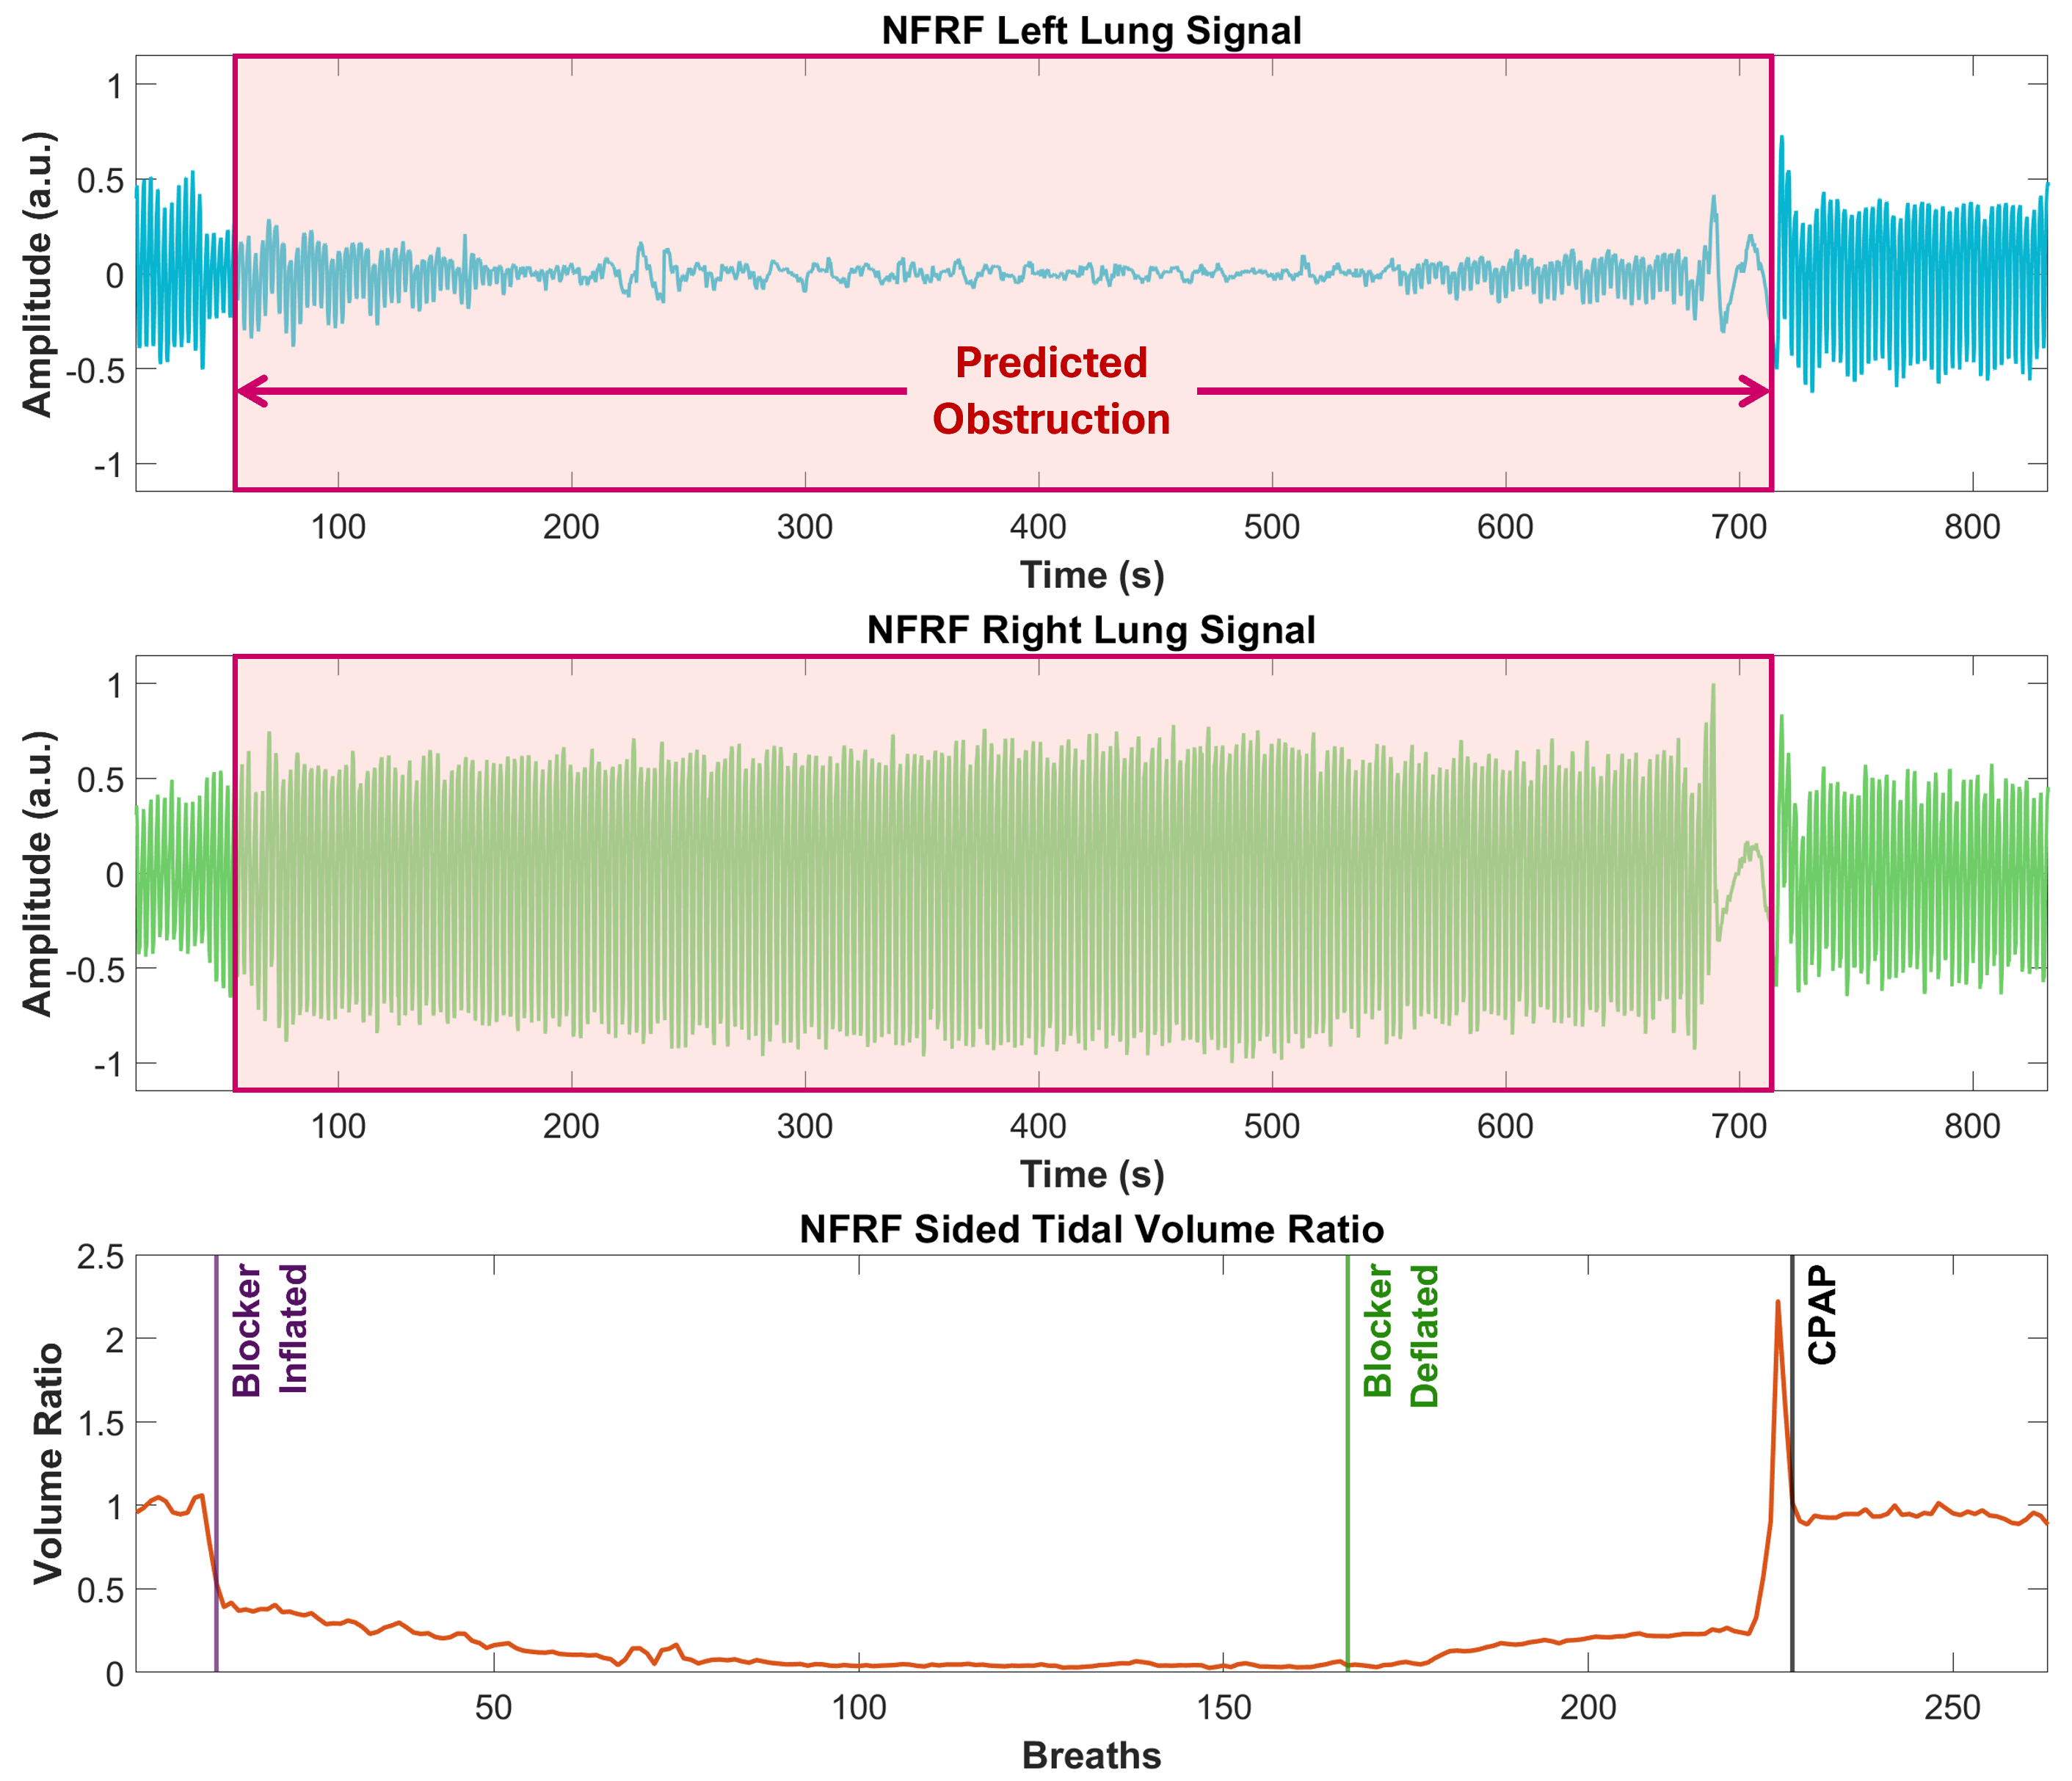
\includegraphics[width=0.98\textwidth]{occlusion_lr.jpg}
    \caption{\textbf{Lung obstruction detection:} The ratio of the estimated left and right lung tidal volume was thresholded to obtain time points of obstruction.}
    \label{fig:occlusion_lr}
\end{figure*}
\sout{By placing the NFRF sensors on either side of the chest, we ensured that each sensor was coupled primarily to the motion of its nearest lung. This enabled us to monitor the continuous change in the tidal volume for each lung independently. The calibration scheme of Eq.~\ref{eq:combine_channels} was modified to use only left and right channels for left and right lung tidal volume estimates, respectively.} \hl{NFRF sensors were placed laterally across the chest, as shown in Fig.~\ref{fig:setup}, with one antenna pair on the left side of the chest and the other antenna pair on the right side, which ensured localized coupling for each antenna pair to the motion of the nearest lung. Every NFRF channel was individually calibrated to the reference spirometer before the start of the procedure, using Eq.~\ref{eq:calibration}. However, instead of using all channels to evaluate the overall tidal volume, we modified Eq.~\ref{eq:combine_channels} to combine channels corresponding to the left antenna pair for left lung tidal volume, and vice versa for the right lung tidal volume.} Fig.~\ref{fig:occlusion_lr} demonstrates how the NFRF volume estimates changed through the occlusion procedure. Since the pig was mechanically ventilated with a constant airflow throughout the intervention, we expect an increase in right lung tidal volume concurrent with a drop in the left lung tidal volumes. We clearly see this behavior in the processed NFRF signals in Fig.~\ref{fig:occlusion_lr}(a). \\
Lung obstruction was detected when the left and right lung tidal volume ratio fell below the empirically chosen threshold of 0.75. The obstruction was considered cleared once the ratio exceeded the threshold again. In order to prevent transients from sudden sensor motion, we monitored the tidal volume ratio over a window of 3 breaths. In the future, when patients are not mechanically ventilated and balloon occluded, the observed change is expected to be much more gradual. Correspondingly, suitable changes to the empirical threshold may be performed to achieve an optimal balance of sensitivity and 1-specificity for the targeted application. In Table \ref{tab:occlusion}, we report the detected occlusion epochs using the above thresholding algorithm. The mean absolute error between actual and predicted onset of obstruction was observed to be 8.29 breaths, owed in part to the 3 breath wait deployed for transient removal. Lung recruitment was observed to show inter-subject differences, with some pigs showing strong recruitment simply after blocker deflation while others requiring the forced CPAP event. Pigs 1-4, which showed recruitment after forced CPAP, had a mean absolute error of 1 breath between the predicted blockage clearance and forced CPAP. Pigs 5 and 7, on the other hand, showed recruitment after blocker deflation with a mean absolute error of 0.5 breaths between the predicted blockage clearance and actual deflation epoch. There were significant external perturbations throughout the protocol for Pig 6, leading to an ill-defined calibration period and spurious detection of clearance of blockage. 
\begin{table}[htbp]
\caption{\textbf{Left lung obstruction detection.} Breaths at which occlusion is detected and cleared.}
    \begin{tabular}{|C{2em} | C{3.5em} | C{4em} | C{3em} | C{4.5em} | C{4.5em}|}
\hline
\multirow{2}{*}{\textbf{Sub.}} & \multicolumn{3}{c|}{\textbf{Ground Truth}} & %
    \multicolumn{2}{c|}{\textbf{Obstruction Detection}}\\
\cline{2-6}
 & \centering \textbf{Blocker Inflated} & \centering \textbf{Blocker Deflated} & \centering \textbf{CPAP} & \centering \textbf{Predicted Start} & \centering \textbf{Predicted End} \tabularnewline
 \hline
1 & 7 & 175 & 209 & 6 & 211 \\ 
 \hline
 2 & 12 & 185 & 272 & 13 & 271\\
 \hline
 3 & 13 & 234 & 296 & 20 & 297\\
 \hline
 4 & 12 & 167 & 228 & 14 & 228 \\
 \hline
 5 & 11 & 428 & 455 & 24 & 428 \\  
 \hline
 6 & 5 & 254 & 319 & 15 & 18 \\  
 \hline
 7 & 29 & 332 & 409 & 53 & 331\\  
 \hline
\end{tabular}
\label{tab:occlusion}
\end{table}

\section{Discussion}
The proposed dual-band NFRF sensor manages to capture unbiased lung tidal volumes to a high accuracy. Our proposed system characterization, based on the near-field backscatter model, shows results in remarkable agreement with the spirometer reference. The limitations of the linear model, Eq.~\ref{eq:lin_vol}, are clearly observed in Fig.~\ref{fig:results}. The standard deviation of NFRF estimates stayed within acceptable limits for tidal volumes up to 450 mL but quickly started deviating at higher values, which is consistent with the sphericity assumption. A nonlinear fitting function could be estimated for individual subjects by performing a multi-point calibration routine. The feasibility of this approach needs to be investigated with a properly designed future study with a larger number of participants. Practically, however, extremely high tidal volumes are primarily observed under mechanical ventilation and are typically avoided to prevent ventilator-induced lung injury, therefore accuracy in these TVs are less critical.\\
We simulated lung collapse by the use of a bronchial blocker whose inflation and deflation were confirmed visually by the use of scopes. While NFRF sensors indicated lung isolation in our study, a true validation requires an imaging reference such as CT-scan or EIT for subsequent studies. We also note that the results of Pig 6 in Table \ref{tab:occlusion} show significant changes from the annotated time stamps. This corresponds to a combination of two factors: a large change in the ambient during the procedure affecting the NFRF calibration, and incomplete intubation. The former indicated the need for external radio isolation which may be ameliorated by the use of more directional antennas. On the other hand, an imaging reference can help provide a more objective ground truth reference than clinical annotations. Although spirometry was regarded as the ground-truth reference in the B\&A analysis, lung volume derived by spirometry also contained noises and errors.  Thus the larger deviation of NFRF from spirometry at large lung volume can contain errors from both instruments.\\
The current NFRF sensing apparatus communicated information to the controlling computer using a wired connection. The entire system can, with a suitable circuit design, be miniaturized into a completely untethered form factor \cite{zhouRadioFrequencyNearFieldSensor2023}. In its current form, sensing antennas were sutured onto the sides of the chests of the pigs. Chest belts may be used as an alternative method for fixing sensors securely \cite{sharmaWearableRadiofrequencySensing2020}. For applications focused more on trends rather than the actual tidal volume, we may deploy a furniture-integrated NFRF system as well \cite{zhangFurnitureIntegratedRespirationSensors2021}.  The above proposed changes in deployment require further investigations into long-term longitudinal consistency, including potential requirements for re-calibration. For the current study, isotropic antennas were utilized as NFRF sensors which, while sufficient for conceptual demonstration, suffer from ambient motion interference. This may be resolved by the use of custom-designed directional or leaky-wave antennas with reflectors to mitigate ambient motion interference. \\
While experts debate on the broad applicability of artificial intelligence to healthcare, there are concerns about the use of black-box algorithms for medical devices \cite{amannExplainabilityArtificialIntelligence2020}. Furthermore, deep neural networks tend to consume significant amounts of processing power and energy, constraining their use for passive and continuous wearables. Classical signal processing algorithms, on the other hand, tend to fare much better in computing power. The use of an interpretable algorithm for combining multi-channel data, using well-defined metrics such as SIR and linearity, can be advantageous for clinical applicability.

\section{Conclusion}
We demonstrated a near-field radio sensing system for continuous monitoring of lung volumes. A stepped change experimental protocol was performed on 8 mechanically ventilated pigs. Data were simultaneously collected from the NFRF system and reference spirometry throughout the procedure. Acquired radio signals were processed, calibrated and benchmarked against reference. We observed excellent agreement between NFRF and reference measurements of lung volumes within reasonable limits. A correlation coefficient of 0.92 was observed in the current study in comparison to 0.81 obtained in prior studies utilizing NFRF sensors for lung tidal volume estimation \cite{sharmaWearableRadiofrequencySensing2020}. \\
We proposed a novel method for detecting sided lung collapse induced by bronchial blockers in the left main bronchus for 7 ventilated pigs. The NFRF sensor can detect obstructions in individual lungs, which is a functional advantage over spirometry which only represents overall airflow. Predicted epochs of airflow cessation and the following lung recruitment after blocker removal were observed to be in close proximity to experimentally observed epochs of lung obstruction. These findings demonstrate the potential of NFRF sensors for continuous, non-invasive monitoring, with significant implications for improving patient care in both acute and chronic respiratory conditions.

\printbibliography

\begin{IEEEbiography}[{
\includegraphics[width=1in,height=1.25in,clip,keepaspectratio]{aakash_corrected2.png}}]{Aakash Kapoor} (Graduate Student Member, IEEE) received the B.Tech degree in electrical engineering from Indian Institute of Technology (IIT) Bombay in 2020, and is currently pursuing the Ph.D. degree in electrical and computer engineering with Cornell University, Ithaca, NY, USA. 
He worked as a Research Engineer at Samsung R\&D Institute, Bangalore, India from 2021 to 2022. His research interesting include biomedical signal processing, non-invasive sensing, sensor design, and machine learning. 
\end{IEEEbiography}

\begin{IEEEbiography}[{
\includegraphics[width=1in,height=1.25in,clip,keepaspectratio]{thomas.jpg}}]{Thomas B. Conroy} received the B.S. degree in electrical engineering from Clarkson University, Potsdam, NY, USA, in 2019, and received the M.S. degree and Ph.D. degree in electrical and computer engineering from Cornell University, Ithaca, NY, USA in 2022 and 2024, respectively. He worked previously at the University of Rochester Heart Research Follow-Up Program on non-invasive arrhythmia detection from 2016 to 2017, and at Johnson \& Johnson Vision in Research and Development in 2018. His research interests include non-invasive biosensing, signal processing, cardiac sensing, and sensor design.
\end{IEEEbiography}

\begin{IEEEbiography}[{
\includegraphics[width=1in,height=1.25in,clip,keepaspectratio]{kapil.jpeg}}]{Kapil Gangwar} (Graduate Student Member, IEEE) was born on April 3, 1996. He is currently pursuing a Ph.D. under the guidance of Prof. Edwin C. Kan in the Department of Electrical and Computer Engineering at Cornell University. His research interests include biomedical sensors and instrumentation, microwave antennas, biomedical imaging, and related techniques. \\
He received his B.Tech. degree in Electronics and Communication Engineering from the Indian Institute of Technology (ISM), Dhanbad, India, in 2019. He completed his Master of Science-thesis degree in Electromagnetics and Microwaves at the University of Alberta, Canada in 2022. His thesis focused on pediatric corpulence and knee osteoarthritis imaging using ultra-wideband radar systems, shaping his current research trajectory. He has authored or coauthored over 16 research papers in international, and national journals and conference proceedings.\\
Mr. Gangwar was a recipient of many prestigious IEEE awards including IEEE Instrumentation \& Measurement Society (IMS) Graduate Fellowship Award 2024, IEEE Antennas \& Propagation Society (AP-S) Fellowship 2023 and 2022, IEEE Microwave Theory \& Technology Society (MTT-S) Undergraduate/Pre-Graduate Scholarship 2022 Cycle -1, IEEE AP-S Eugene F. Knott Memorial Pre-Doctoral Research Grant Award 2021, and many other scholarships at the University of Alberta.
\end{IEEEbiography}

\begin{IEEEbiography}[{
\includegraphics[width=1in,height=1.25in,clip,keepaspectratio]{edwin.png}}]{Edwin C. Kan} (Senior Member, IEEE) received a B.S. degree from National Taiwan University in 1984, and M.S. and Ph.D. degrees from the University of Illinois, Urbana-Champaign in 1988 and 1992, respectively, all in Electrical Engineering. In January 1992, he joined Dawn Technologies, Sunnyvale CA, as a CAD Engineer. He was then with Stanford University as a Research Associate from 1994 to 1997. In 1997, he started as an Assistant Professor in School of Electrical and Computer Engineering, Cornell University, Ithaca, NY, where he is now a professor. His research interests include RF biosensors, RFID, RF imaging, CMOS technology, flash memory, molecular sensors, and technology computer-aided design (TCAD).
\end{IEEEbiography}

\begin{IEEEbiography}[{
\includegraphics[width=1in,height=1.25in,clip,keepaspectratio]{joaquin.jpg}}]{Joaquin Araos} received his degree in veterinary medicine from Universidad Mayor, Chile, in 2007. He completed a residency in veterinary anesthesiology at the University of Pennsylvania, Philadelphia, in 2012, after which he obtained DACVAA certification. In 2017, he earned a Ph.D. in Clinical Sciences from Pontificia Universidad Católica de Chile. He then joined the University of Montreal as a clinical anesthesiologist. In 2019, he became a lecturer in anesthesiology at Cornell University, and as of July 2024, he is an associate professor on a tenure track. His research interests include heart-lung interactions, acute respiratory distress syndrome, extracorporeal support, and cardiopulmonary monitoring methods.
\end{IEEEbiography}

\end{document}
